\documentclass[]{book}
\usepackage{lmodern}
\usepackage{amssymb,amsmath}
\usepackage{ifxetex,ifluatex}
\usepackage{fixltx2e} % provides \textsubscript
\ifnum 0\ifxetex 1\fi\ifluatex 1\fi=0 % if pdftex
  \usepackage[T1]{fontenc}
  \usepackage[utf8]{inputenc}
\else % if luatex or xelatex
  \ifxetex
    \usepackage{mathspec}
  \else
    \usepackage{fontspec}
  \fi
  \defaultfontfeatures{Ligatures=TeX,Scale=MatchLowercase}
\fi
% use upquote if available, for straight quotes in verbatim environments
\IfFileExists{upquote.sty}{\usepackage{upquote}}{}
% use microtype if available
\IfFileExists{microtype.sty}{%
\usepackage[]{microtype}
\UseMicrotypeSet[protrusion]{basicmath} % disable protrusion for tt fonts
}{}
\PassOptionsToPackage{hyphens}{url} % url is loaded by hyperref
\usepackage[unicode=true]{hyperref}
\hypersetup{
            pdftitle={Wearables Book},
            pdfauthor={Merck and Data Mine Corporate Partnership Team},
            pdfborder={0 0 0},
            breaklinks=true}
\urlstyle{same}  % don't use monospace font for urls
\usepackage{natbib}
\bibliographystyle{apalike}
\usepackage{color}
\usepackage{fancyvrb}
\newcommand{\VerbBar}{|}
\newcommand{\VERB}{\Verb[commandchars=\\\{\}]}
\DefineVerbatimEnvironment{Highlighting}{Verbatim}{commandchars=\\\{\}}
% Add ',fontsize=\small' for more characters per line
\usepackage{framed}
\definecolor{shadecolor}{RGB}{248,248,248}
\newenvironment{Shaded}{\begin{snugshade}}{\end{snugshade}}
\newcommand{\KeywordTok}[1]{\textcolor[rgb]{0.13,0.29,0.53}{\textbf{#1}}}
\newcommand{\DataTypeTok}[1]{\textcolor[rgb]{0.13,0.29,0.53}{#1}}
\newcommand{\DecValTok}[1]{\textcolor[rgb]{0.00,0.00,0.81}{#1}}
\newcommand{\BaseNTok}[1]{\textcolor[rgb]{0.00,0.00,0.81}{#1}}
\newcommand{\FloatTok}[1]{\textcolor[rgb]{0.00,0.00,0.81}{#1}}
\newcommand{\ConstantTok}[1]{\textcolor[rgb]{0.00,0.00,0.00}{#1}}
\newcommand{\CharTok}[1]{\textcolor[rgb]{0.31,0.60,0.02}{#1}}
\newcommand{\SpecialCharTok}[1]{\textcolor[rgb]{0.00,0.00,0.00}{#1}}
\newcommand{\StringTok}[1]{\textcolor[rgb]{0.31,0.60,0.02}{#1}}
\newcommand{\VerbatimStringTok}[1]{\textcolor[rgb]{0.31,0.60,0.02}{#1}}
\newcommand{\SpecialStringTok}[1]{\textcolor[rgb]{0.31,0.60,0.02}{#1}}
\newcommand{\ImportTok}[1]{#1}
\newcommand{\CommentTok}[1]{\textcolor[rgb]{0.56,0.35,0.01}{\textit{#1}}}
\newcommand{\DocumentationTok}[1]{\textcolor[rgb]{0.56,0.35,0.01}{\textbf{\textit{#1}}}}
\newcommand{\AnnotationTok}[1]{\textcolor[rgb]{0.56,0.35,0.01}{\textbf{\textit{#1}}}}
\newcommand{\CommentVarTok}[1]{\textcolor[rgb]{0.56,0.35,0.01}{\textbf{\textit{#1}}}}
\newcommand{\OtherTok}[1]{\textcolor[rgb]{0.56,0.35,0.01}{#1}}
\newcommand{\FunctionTok}[1]{\textcolor[rgb]{0.00,0.00,0.00}{#1}}
\newcommand{\VariableTok}[1]{\textcolor[rgb]{0.00,0.00,0.00}{#1}}
\newcommand{\ControlFlowTok}[1]{\textcolor[rgb]{0.13,0.29,0.53}{\textbf{#1}}}
\newcommand{\OperatorTok}[1]{\textcolor[rgb]{0.81,0.36,0.00}{\textbf{#1}}}
\newcommand{\BuiltInTok}[1]{#1}
\newcommand{\ExtensionTok}[1]{#1}
\newcommand{\PreprocessorTok}[1]{\textcolor[rgb]{0.56,0.35,0.01}{\textit{#1}}}
\newcommand{\AttributeTok}[1]{\textcolor[rgb]{0.77,0.63,0.00}{#1}}
\newcommand{\RegionMarkerTok}[1]{#1}
\newcommand{\InformationTok}[1]{\textcolor[rgb]{0.56,0.35,0.01}{\textbf{\textit{#1}}}}
\newcommand{\WarningTok}[1]{\textcolor[rgb]{0.56,0.35,0.01}{\textbf{\textit{#1}}}}
\newcommand{\AlertTok}[1]{\textcolor[rgb]{0.94,0.16,0.16}{#1}}
\newcommand{\ErrorTok}[1]{\textcolor[rgb]{0.64,0.00,0.00}{\textbf{#1}}}
\newcommand{\NormalTok}[1]{#1}
\usepackage{longtable,booktabs}
% Fix footnotes in tables (requires footnote package)
\IfFileExists{footnote.sty}{\usepackage{footnote}\makesavenoteenv{long table}}{}
\usepackage{graphicx,grffile}
\makeatletter
\def\maxwidth{\ifdim\Gin@nat@width>\linewidth\linewidth\else\Gin@nat@width\fi}
\def\maxheight{\ifdim\Gin@nat@height>\textheight\textheight\else\Gin@nat@height\fi}
\makeatother
% Scale images if necessary, so that they will not overflow the page
% margins by default, and it is still possible to overwrite the defaults
% using explicit options in \includegraphics[width, height, ...]{}
\setkeys{Gin}{width=\maxwidth,height=\maxheight,keepaspectratio}
\IfFileExists{parskip.sty}{%
\usepackage{parskip}
}{% else
\setlength{\parindent}{0pt}
\setlength{\parskip}{6pt plus 2pt minus 1pt}
}
\setlength{\emergencystretch}{3em}  % prevent overfull lines
\providecommand{\tightlist}{%
  \setlength{\itemsep}{0pt}\setlength{\parskip}{0pt}}
\setcounter{secnumdepth}{5}
% Redefines (sub)paragraphs to behave more like sections
\ifx\paragraph\undefined\else
\let\oldparagraph\paragraph
\renewcommand{\paragraph}[1]{\oldparagraph{#1}\mbox{}}
\fi
\ifx\subparagraph\undefined\else
\let\oldsubparagraph\subparagraph
\renewcommand{\subparagraph}[1]{\oldsubparagraph{#1}\mbox{}}
\fi

% set default figure placement to htbp
\makeatletter
\def\fps@figure{htbp}
\makeatother

\usepackage{booktabs}
\usepackage{amsthm}
\makeatletter
\def\thm@space@setup{%
  \thm@preskip=8pt plus 2pt minus 4pt
  \thm@postskip=\thm@preskip
}
\makeatother

\title{Wearables Book}
\author{Merck and Data Mine Corporate Partnership Team}
\date{2020-07-28}

\begin{document}
\maketitle

{
\setcounter{tocdepth}{1}
\tableofcontents
}
\chapter{Book Overview}\label{book-overview}

A foundation of knowledge in the data sciences can prove advantageous
for almost all scientists. Often, however, understanding the
fundamentals of any new skill lacking proper instruction or recourses
can be difficult. With ample guidance, all can develop a base knowledge
of Data Science that can grow and provide new skills for improved
research experiences.

The sets of instruction, examples, and tutorials in this walk-through
are specifically designed for Merck Technology and can be distributed to
Merck Scientists. The walk-through will be tailored to the needs of the
pharmaceutical industry and will relate to work being done at Merck.

In this walkthrough, a complete, end-to-end, project will be outlined
with instructional and applicational opportunities throughout.

\chapter{Data Science Overview}\label{intro}

Data Science is an interdisciplinary field aimed to extract insight from
structured and unstructured data. An intersection between computing,
statistics, mathematics, and domain application, data science reveals
new meaning to the extreme amounts of data being collected and stored
every day.

Some of the foundational skills that the data sciences require include
basic computing and data analysis knowledge. A range of technologies are
used daily by data scientists, including Python, R, Hadoop, Bash, and
more. Statistical concepts like descriptive statistics, probability,
Bayesian theory, and modeling are used in combination with the
previously mentioned technologies to gain insight from data.

\chapter{Project Introduction}\label{project-introduction}

An end-to-end project will be outlined in the remainder of the text.
Primary concepts included are data capture, data visualization, and
client-server communication. The technologies covered will include
Python, Bash, SQL, R, and React Native along with many useful packages
and dependencies.

Throughout each section of the text, there will be an introduction to a
new technology. Basic programming skills and logic explanation related
to the technology will be covered within this section. Using the skills
taught, the walkthrough section will follow, where instruction related
to the overall project will be given.

The project being taught in this text is a data capture project that
will evolve into a basic mobile application. Using Fitbit technology,
users are collecting massive amounts of biometric data that, if captured
properly, can be used to benefit pharmaceutical research. Patient
activity, heart, sleep, and weight data can all be captured seamlessly.
The medicinal benefits are great with a tool like this. It is through
simple computing and foundational data science topics that a pipeline
and tool can be engineered.

\chapter{Using Git and GitHub}\label{using-git-and-github}

\section{Git and GitHub Overview}\label{git-and-github-overview}

Git is a distributed version-control system for tracking changes in
source code during software development. It is designed for coordinating
work among programmers, but it can be used to track changes in any set
of files. Its goals include speed, data integrity, and support for
distributed, non-linear workflows.

GitHub serves as a web-based interface for Git while also providing many
otehr valuable features for version control and collaboration.

Downloading Git can be done at \url{https://git-scm.com/downloads}.
GitHub is free to create to create an account at
\url{https://github.com/}.

During this section, we will work through the basics of Git and GitHub!

\section{Important Git Commands}\label{important-git-commands}

\begin{Shaded}
\begin{Highlighting}[]
\FunctionTok{git}\NormalTok{ clone                       # clone a repository into a new directory}
\end{Highlighting}
\end{Shaded}

\begin{Shaded}
\begin{Highlighting}[]
\FunctionTok{git}\NormalTok{ init                        # initialize local directory as a git repository}
\end{Highlighting}
\end{Shaded}

\begin{Shaded}
\begin{Highlighting}[]
\FunctionTok{git}\NormalTok{ add .                       # add files to local repository}
\end{Highlighting}
\end{Shaded}

\begin{Shaded}
\begin{Highlighting}[]
\FunctionTok{git}\NormalTok{ commit- m “commit message”  # commit files you staged in local repository}
\end{Highlighting}
\end{Shaded}

\begin{Shaded}
\begin{Highlighting}[]
\FunctionTok{git}\NormalTok{ remote add origin URL           # sets remote location of Github repository with URL}
\end{Highlighting}
\end{Shaded}

\begin{Shaded}
\begin{Highlighting}[]
\FunctionTok{git}\NormalTok{ remote -v                         # verifies remote location}
\end{Highlighting}
\end{Shaded}

\begin{Shaded}
\begin{Highlighting}[]
\FunctionTok{git}\NormalTok{ push                                  # pushes changes from local repository to remote repository }
\end{Highlighting}
\end{Shaded}

\begin{Shaded}
\begin{Highlighting}[]
\FunctionTok{git}\NormalTok{ branch                            # check which branch you are currently working on}
\end{Highlighting}
\end{Shaded}

\begin{Shaded}
\begin{Highlighting}[]
\FunctionTok{git}\NormalTok{ checkout branch-name            # change branches}
\end{Highlighting}
\end{Shaded}

\begin{Shaded}
\begin{Highlighting}[]
\FunctionTok{git}\NormalTok{ checkout -b branch-name     # create a new branch if branch-name does not exist }
\end{Highlighting}
\end{Shaded}

\begin{Shaded}
\begin{Highlighting}[]
\FunctionTok{git}\NormalTok{ status                            # displays state of working directory and changed states}
\end{Highlighting}
\end{Shaded}

\begin{Shaded}
\begin{Highlighting}[]
\FunctionTok{git}\NormalTok{ pull                                  # update local version of a repository from remote repository}
\end{Highlighting}
\end{Shaded}

\section{Git and GitHub Simple
Walkthrough}\label{git-and-github-simple-walkthrough}

Let's learn some basics of Git and GitHub through an example.

To start, make a new directory and cd into it.

\begin{Shaded}
\begin{Highlighting}[]
\FunctionTok{mkdir}\NormalTok{ myGitTutorial}

\BuiltInTok{cd}\NormalTok{ myGitTutorial}
\end{Highlighting}
\end{Shaded}

Now, create a readme file and add a description within our new
directory.

\begin{Shaded}
\begin{Highlighting}[]
\FunctionTok{touch}\NormalTok{ readme.md}

\BuiltInTok{echo}\NormalTok{ this is the read me for my Git tutorial }\OperatorTok{>}\NormalTok{ readme.md}
\end{Highlighting}
\end{Shaded}

Initialize the Git repository.

\begin{Shaded}
\begin{Highlighting}[]
\FunctionTok{git}\NormalTok{ init}
\end{Highlighting}
\end{Shaded}

Add and commit files to local git repository.

\begin{Shaded}
\begin{Highlighting}[]
\FunctionTok{git}\NormalTok{ add .}

\FunctionTok{git}\NormalTok{ commit -m “initial commit.”}
\end{Highlighting}
\end{Shaded}

Now, if neeeded, create a GitHub account and then create a new
repository.

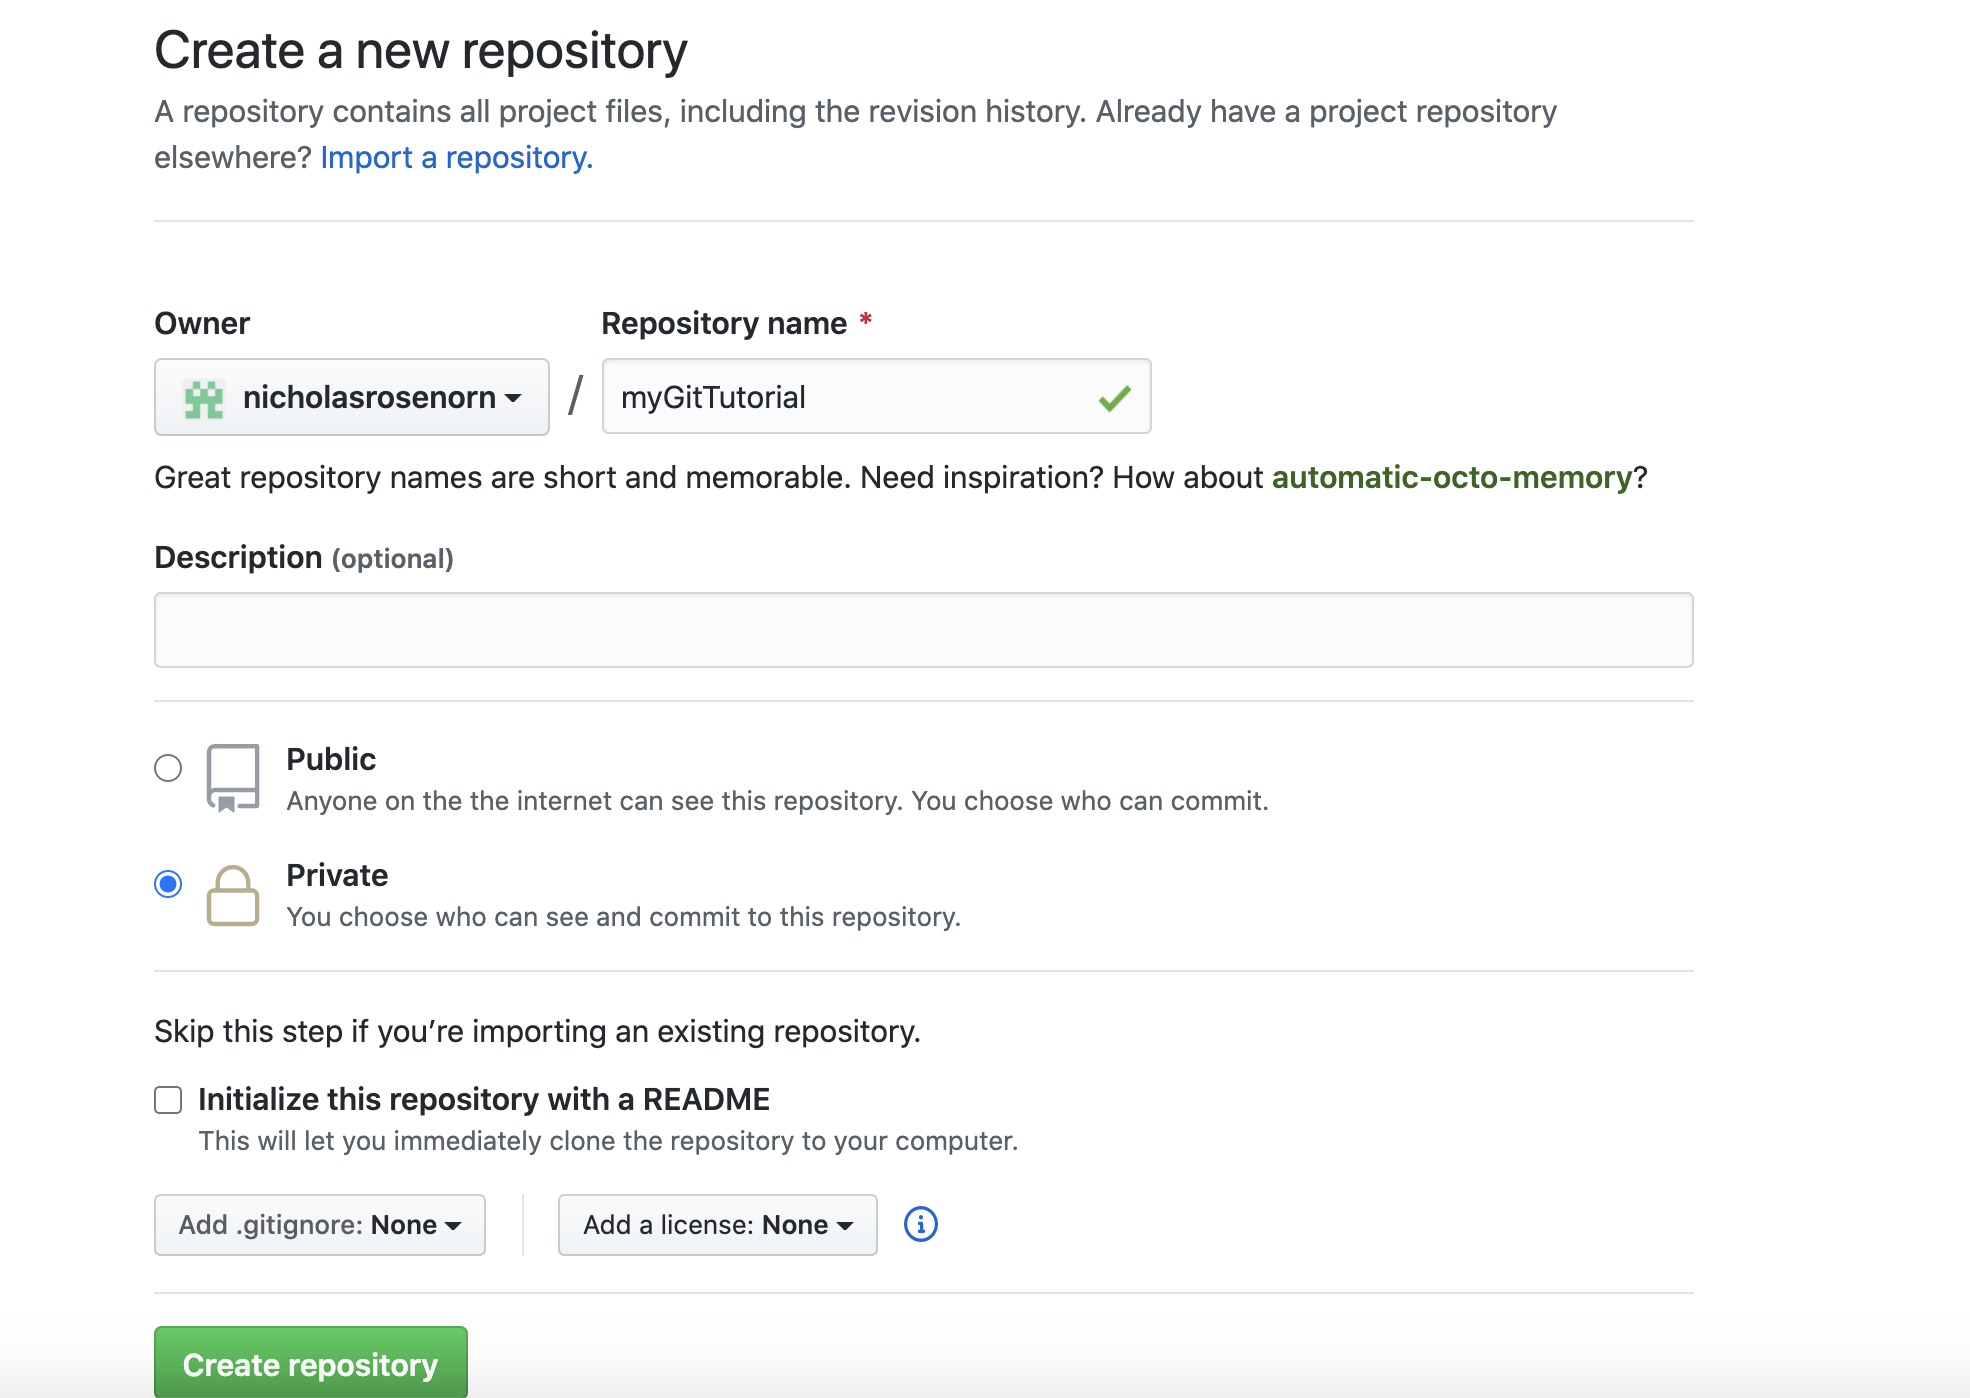
\includegraphics[width=0.40000\textwidth]{images/create new git repo.png}

Back in command line, set remote location of repository

\begin{Shaded}
\begin{Highlighting}[]
\FunctionTok{git}\NormalTok{ remote add origin link/of/your/GitHub/repo}
\end{Highlighting}
\end{Shaded}

Now, we can push contents to the remote repository on GitHub.

\begin{Shaded}
\begin{Highlighting}[]
\FunctionTok{git}\NormalTok{ push -u origin master}
\end{Highlighting}
\end{Shaded}

The repository is now set up and can be viewed in Github! You will see
the readme file we created in the repo.

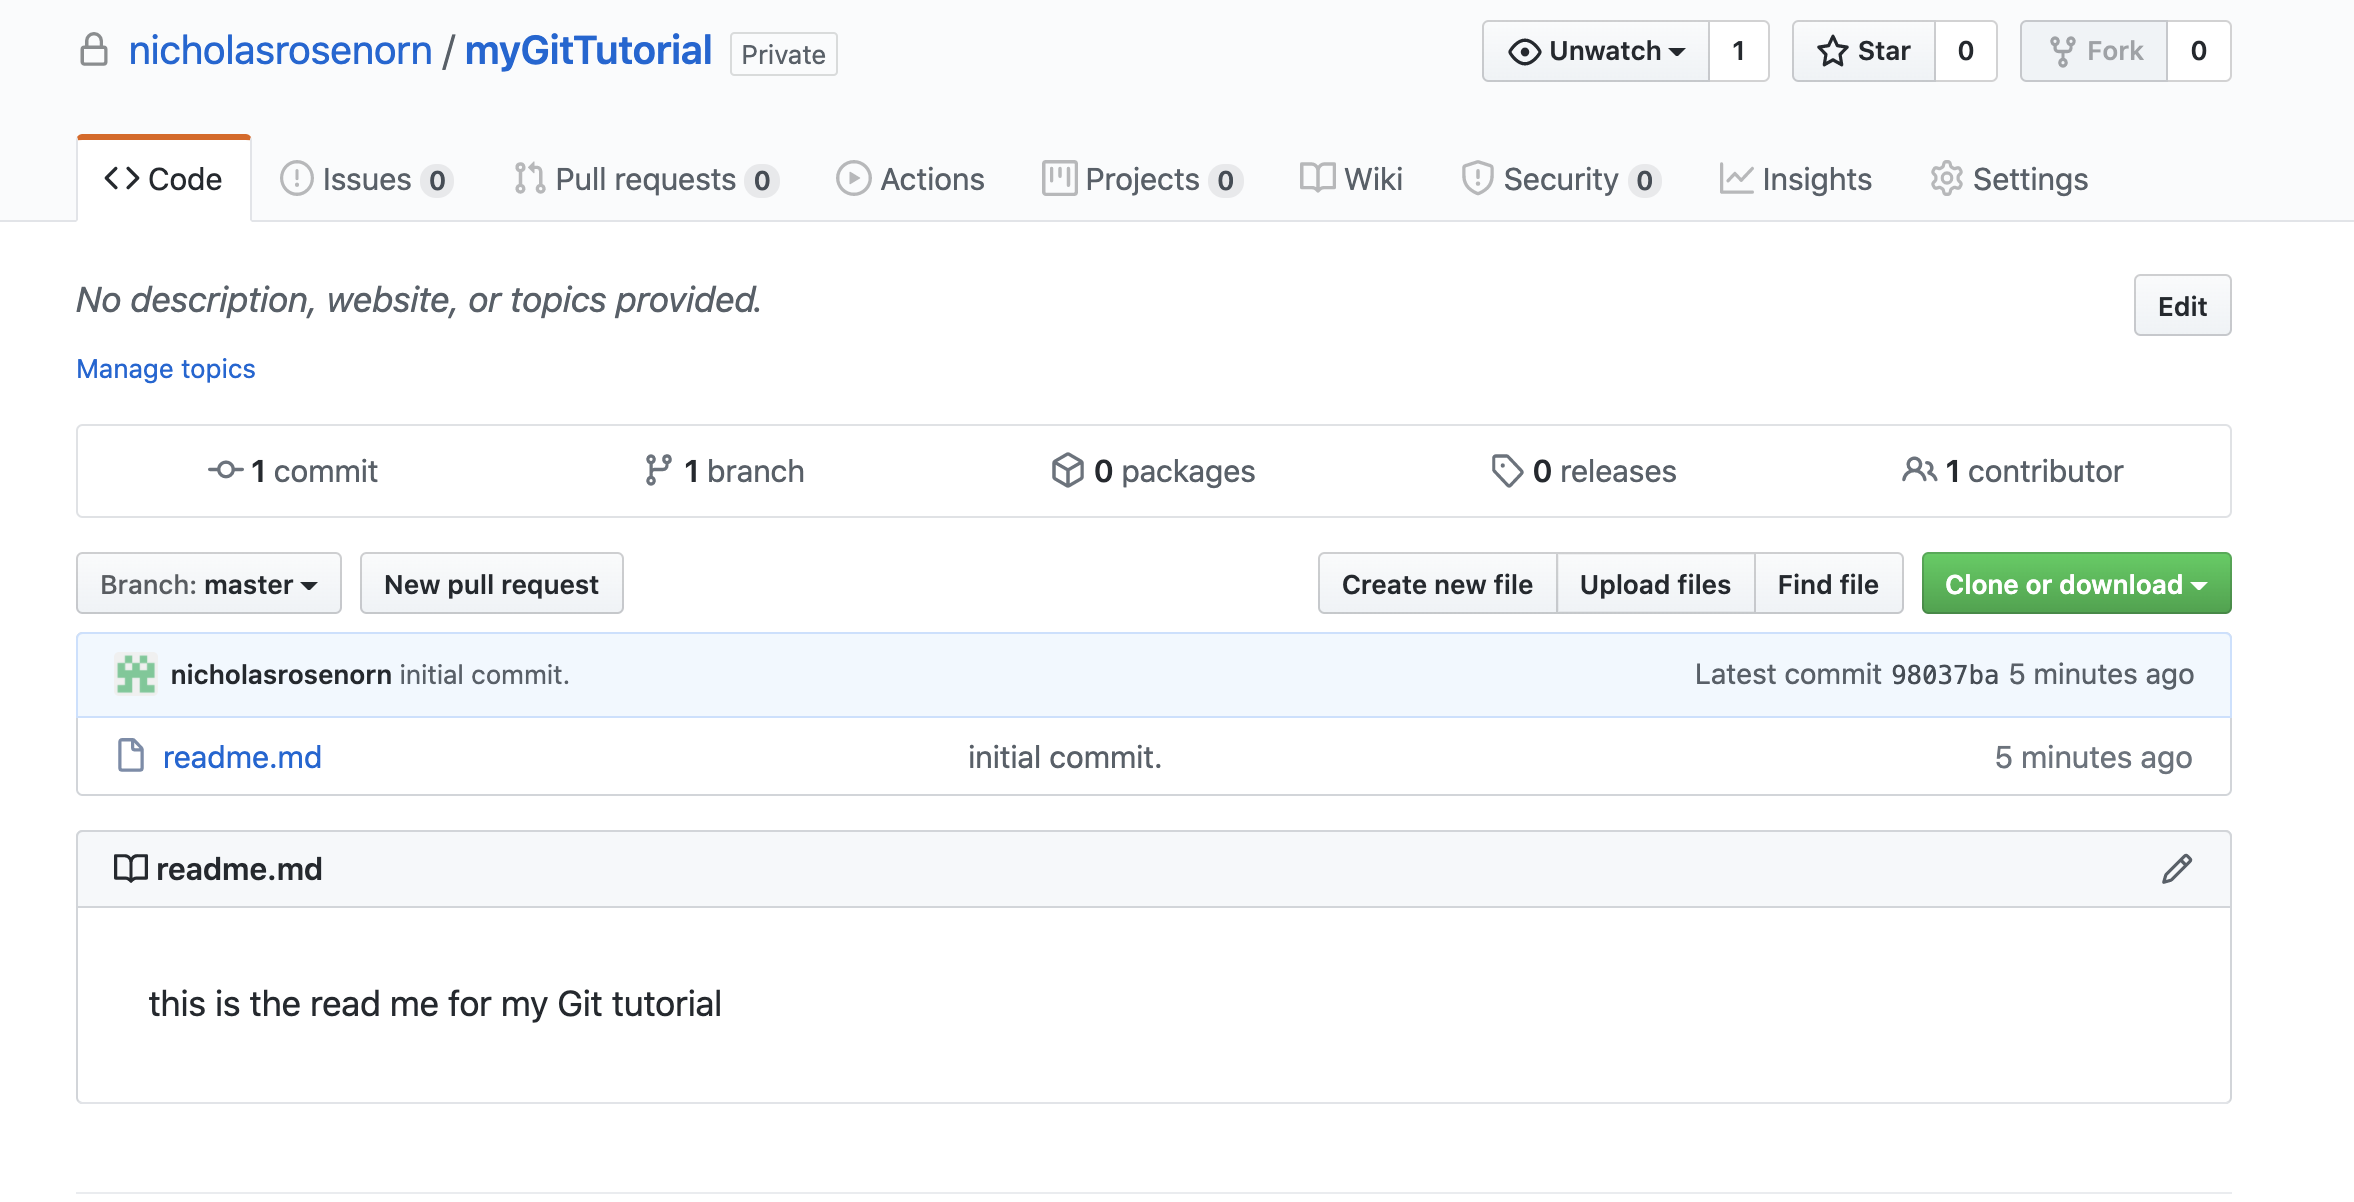
\includegraphics[width=0.40000\textwidth]{images/github view.png}

Next, we can create a new branch.

\begin{Shaded}
\begin{Highlighting}[]
\FunctionTok{git}\NormalTok{ checkout -b tutorial-branch}
\end{Highlighting}
\end{Shaded}

Make a new file in the tutorial branch

\begin{Shaded}
\begin{Highlighting}[]
\FunctionTok{touch}\NormalTok{ branch.txt}
\BuiltInTok{echo}\NormalTok{ this is for the tutorial branch }\OperatorTok{>}\NormalTok{ branch.txt}
\end{Highlighting}
\end{Shaded}

Stage and commit files to branch.

\begin{Shaded}
\begin{Highlighting}[]
\FunctionTok{git}\NormalTok{ add .}

\FunctionTok{git}\NormalTok{ commit -m }\StringTok{"txt file to branch"}
\end{Highlighting}
\end{Shaded}

Push staged files to branch.

\begin{Shaded}
\begin{Highlighting}[]
\FunctionTok{git}\NormalTok{ push --set-upstream origin tutorial-branch}
\end{Highlighting}
\end{Shaded}

When we return to github we will notice that there are two branches!

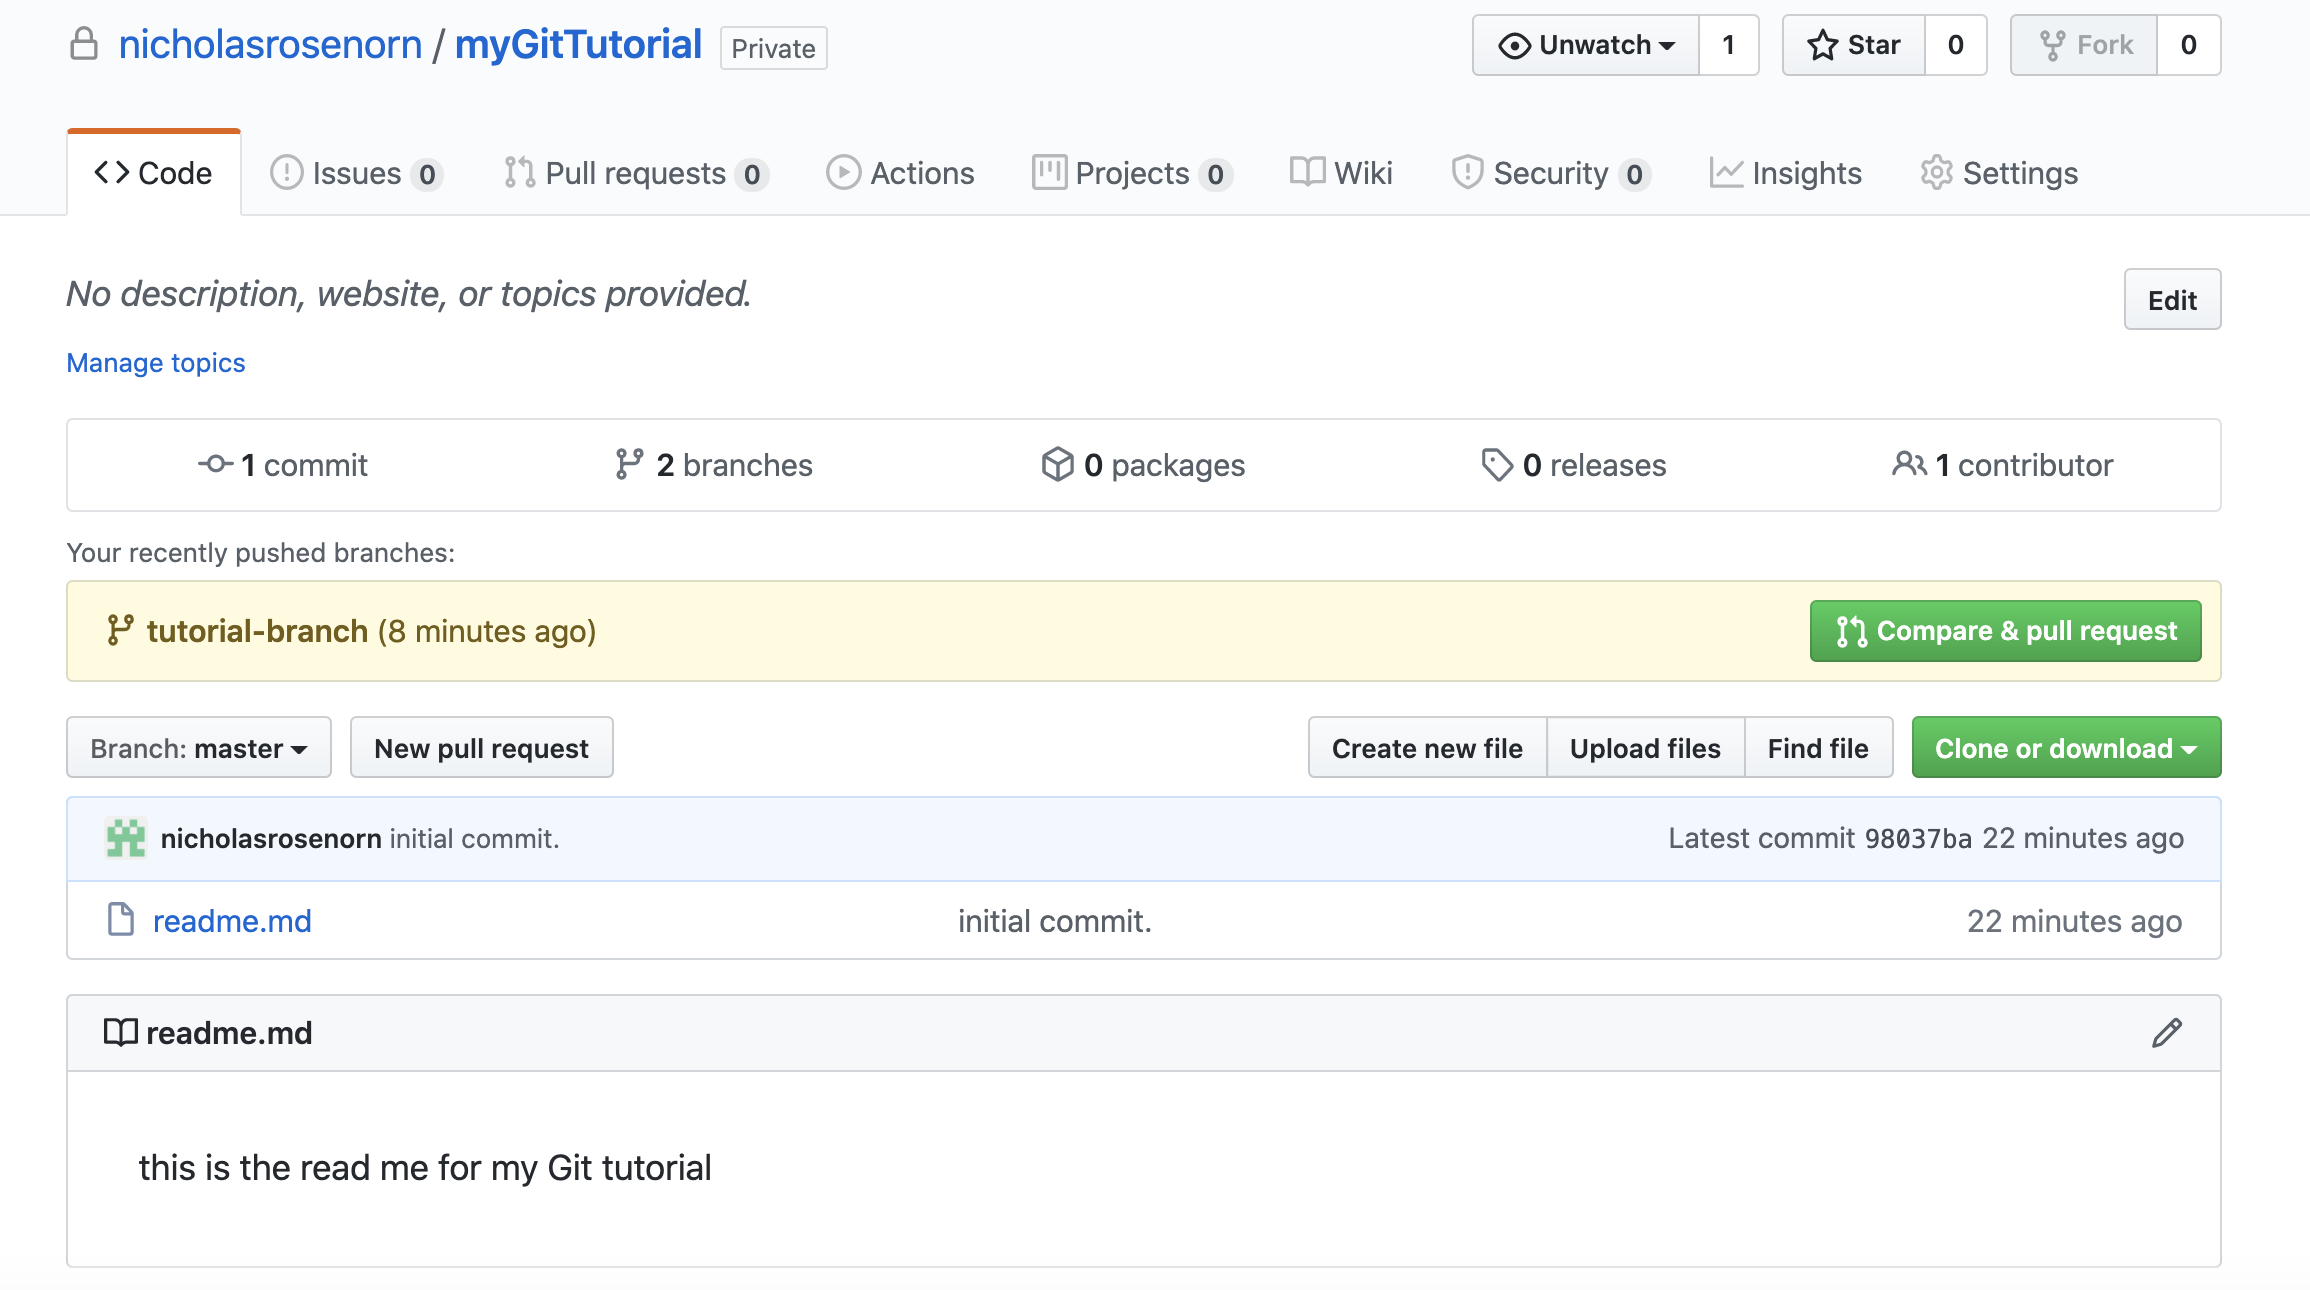
\includegraphics[width=0.40000\textwidth]{images/branch.png}

Notice that the master branch does not have the newly created branch.txt
file. If we navigate to tutorial-branch, we will see the branch.txt
file!

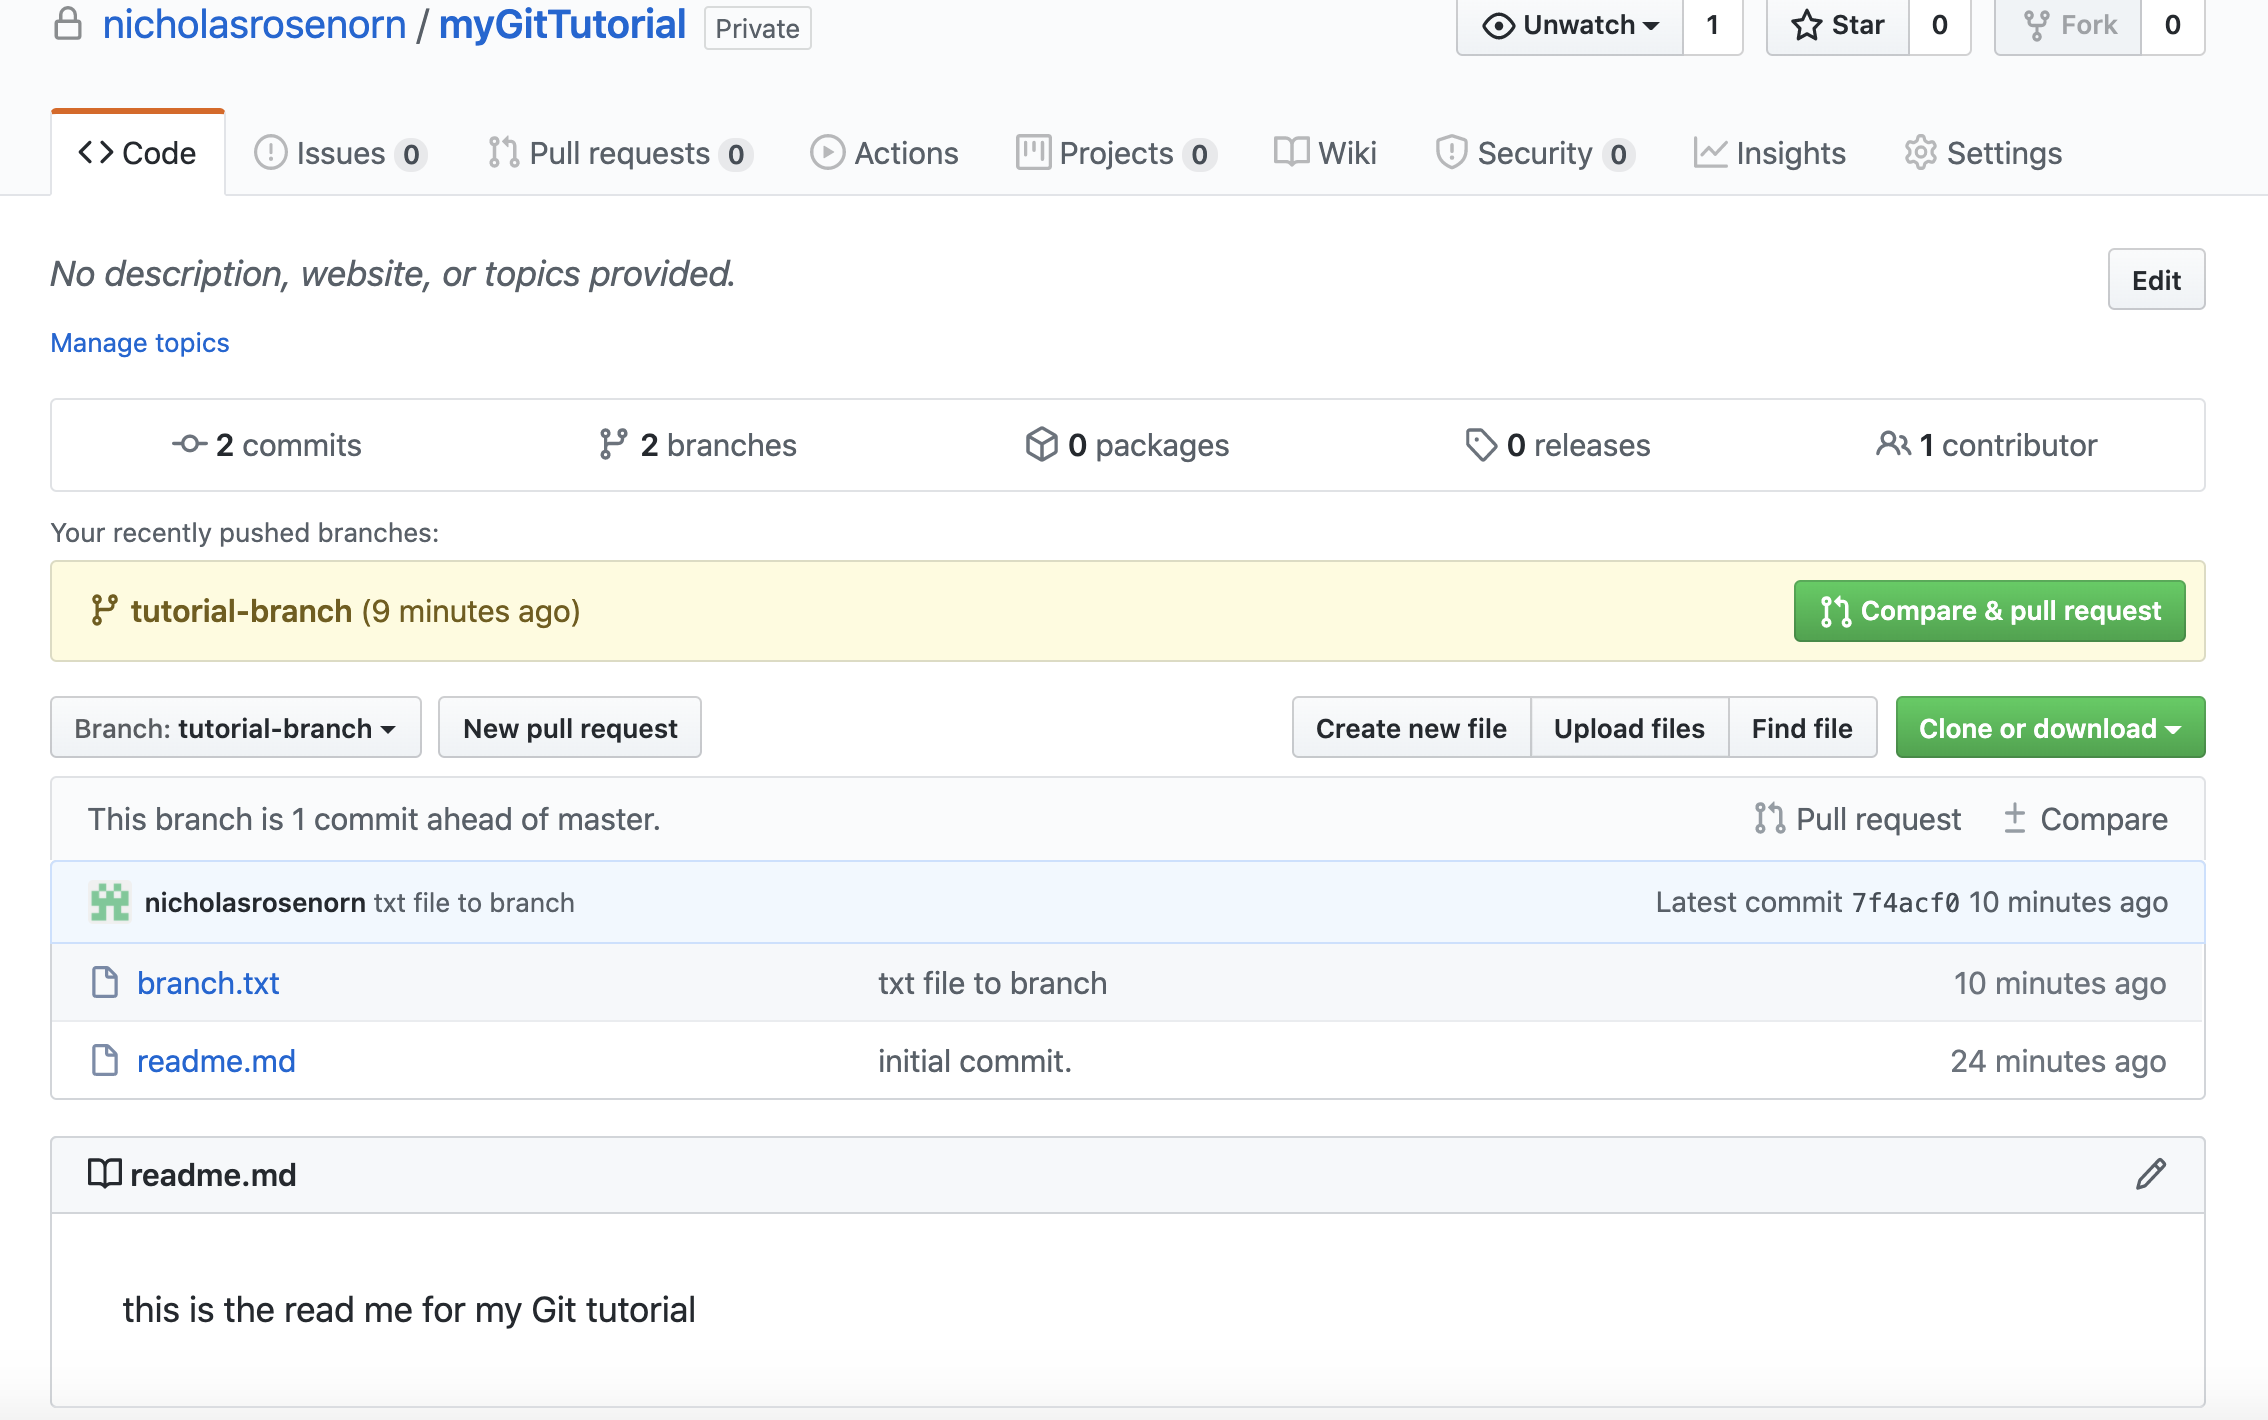
\includegraphics[width=0.40000\textwidth]{images/commit.png}

Let's update the master branch with the added files from the branch. To
update the master branch, we will need to create a pull request.

Click the green button that says `compare and pull request'.

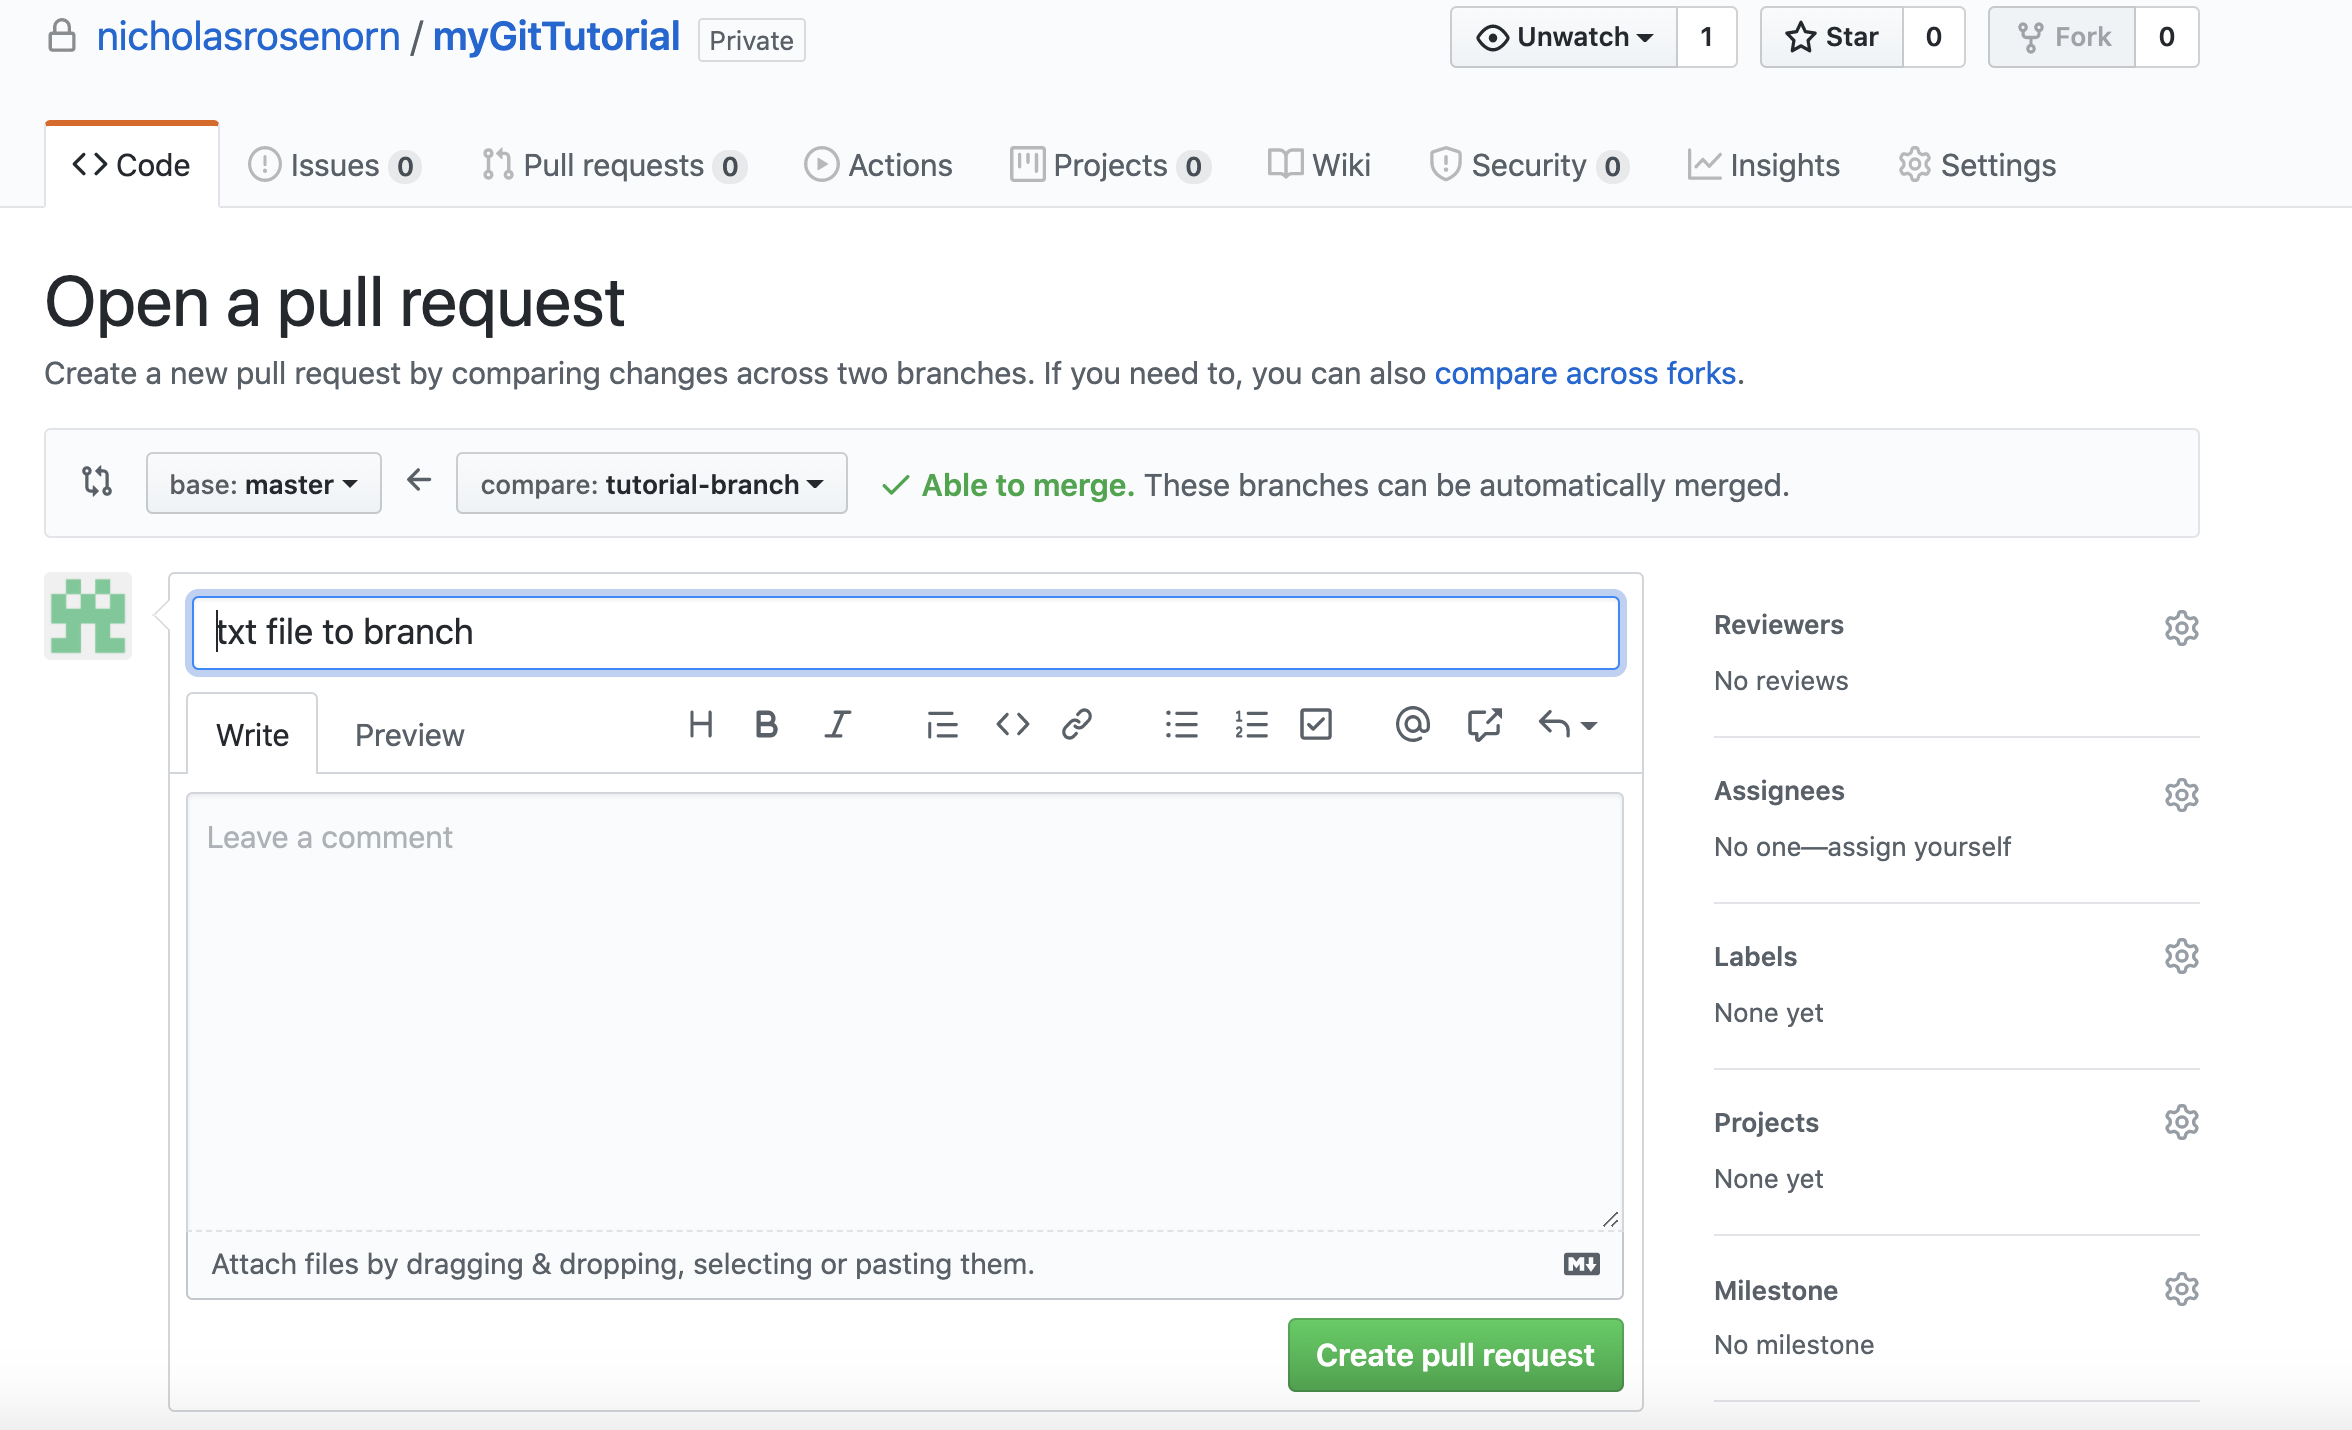
\includegraphics[width=0.40000\textwidth]{images/pull.png}

Then, click `create pull request'. Notice how there are no conflicts
with the master branch!

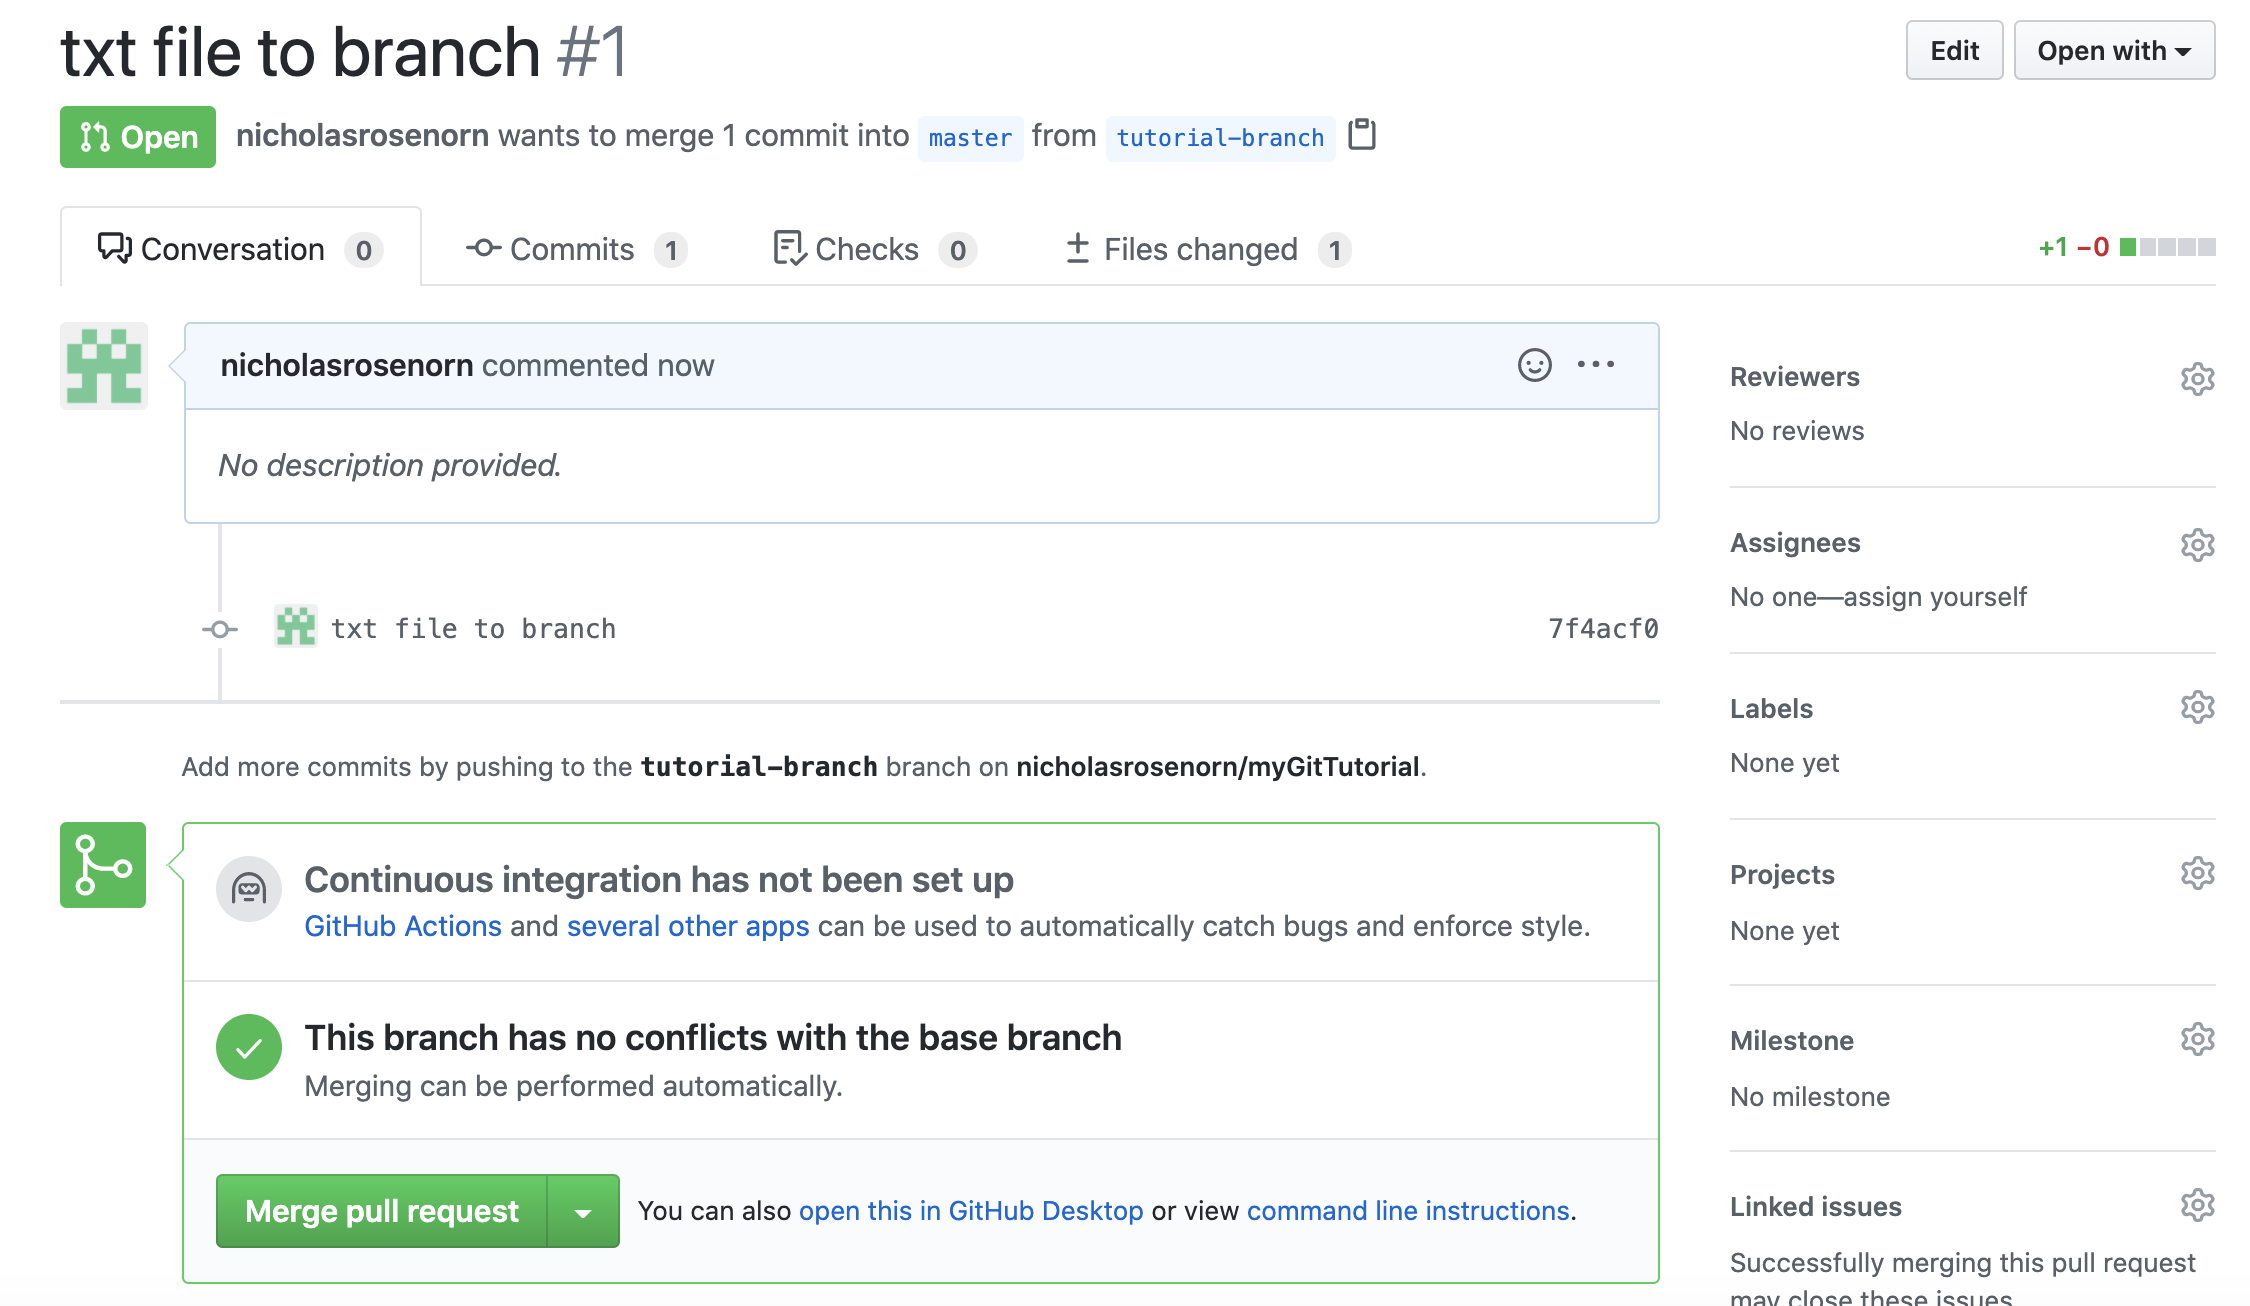
\includegraphics[width=0.40000\textwidth]{images/merge.png}

Now click `Merge pull request' and then `confirm merge'.

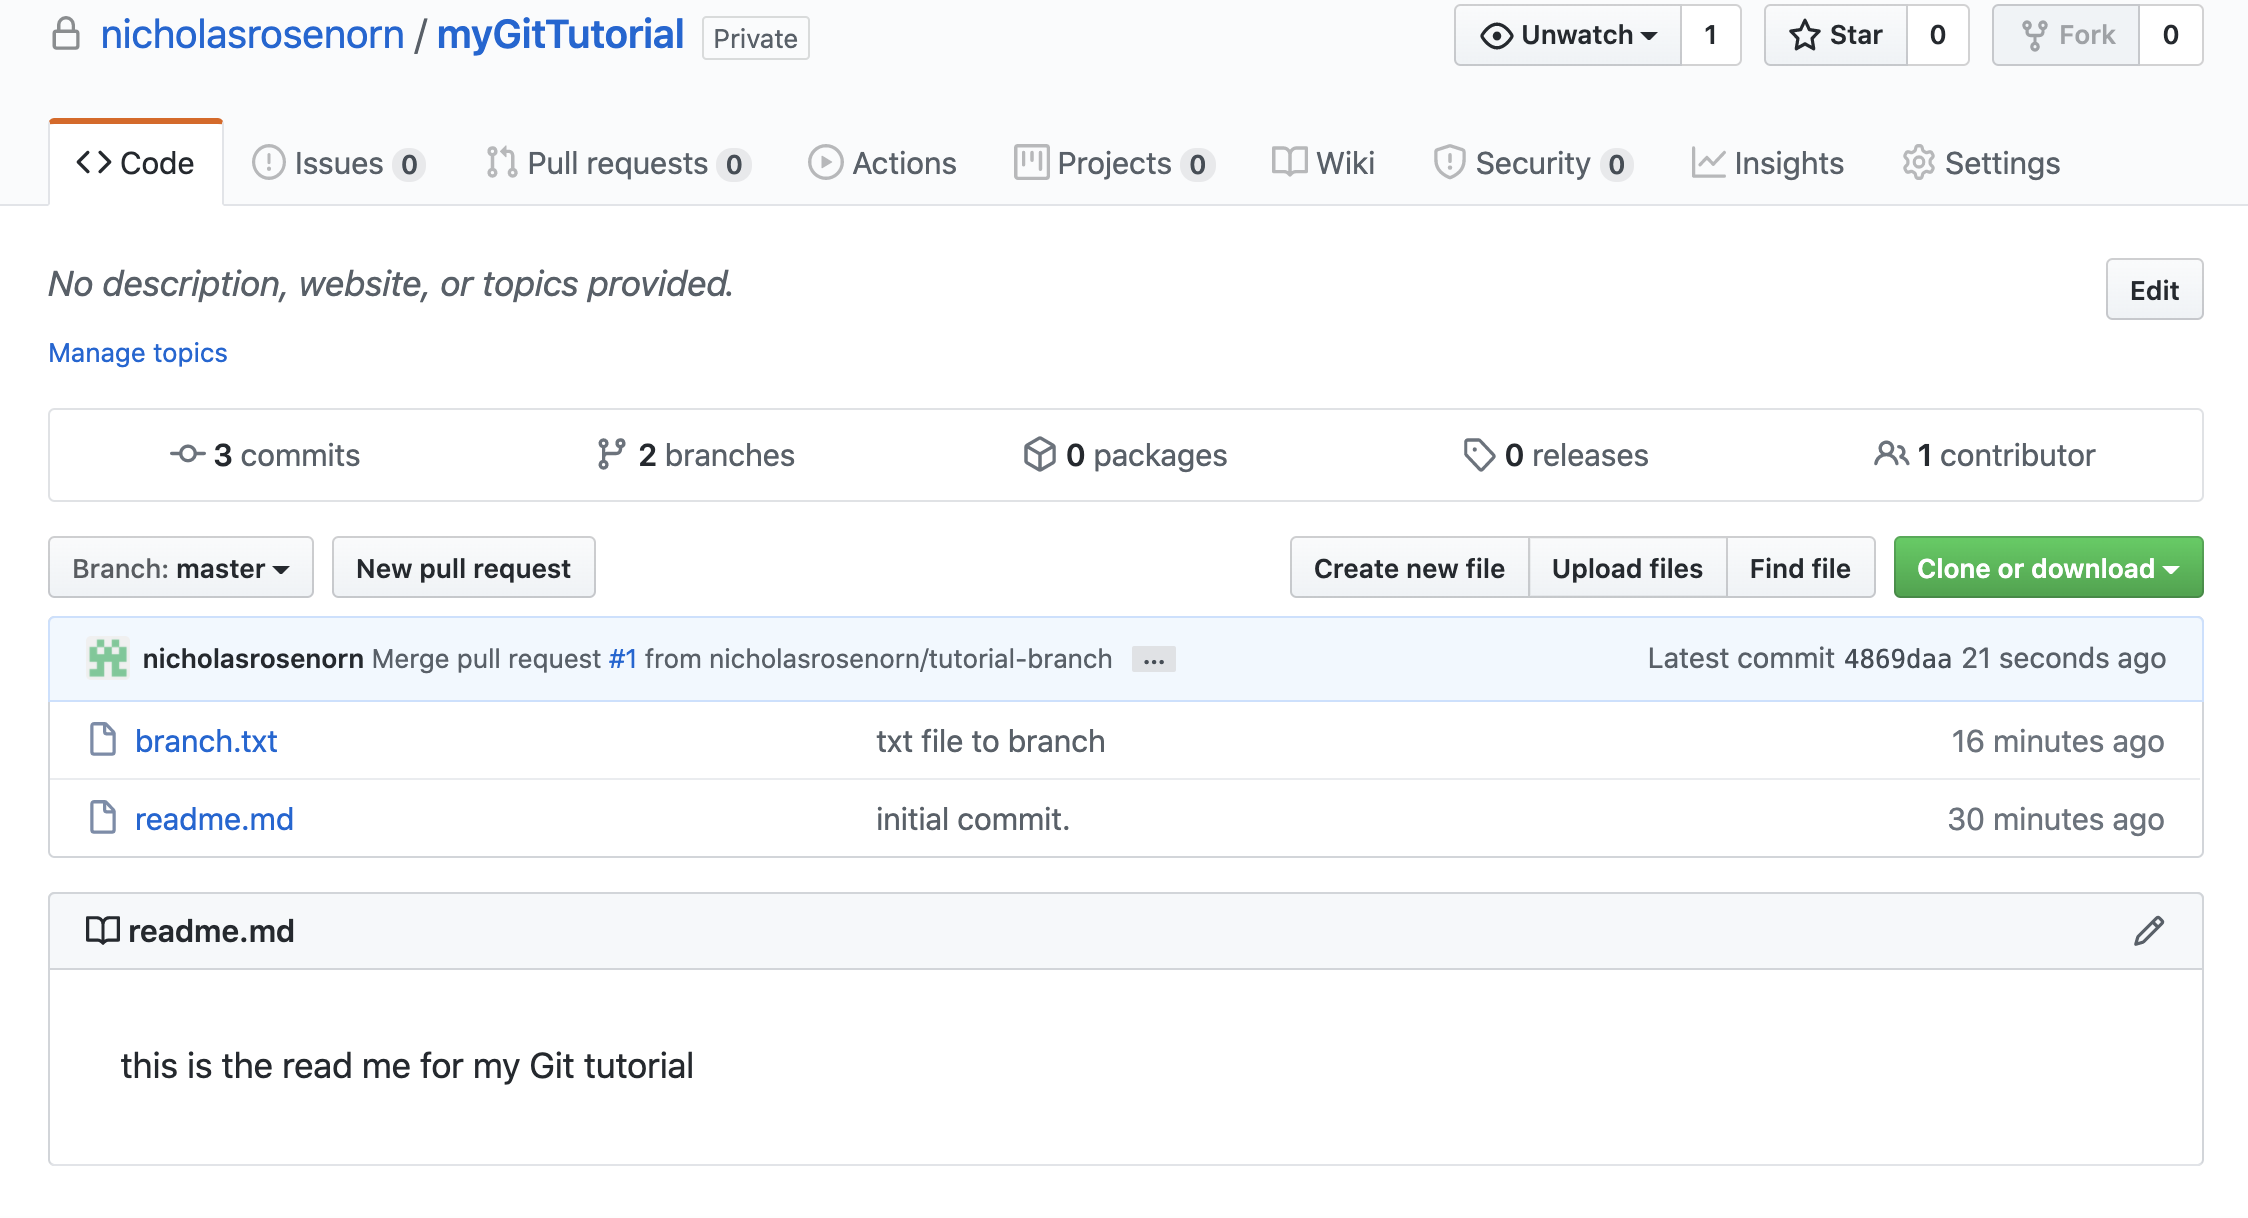
\includegraphics[width=0.40000\textwidth]{images/final.png}

Once the merge is done processing we can return to the master branch and
we will see that branch.txt is now available on the master!

\chapter{Fitbit Technology}\label{fitbit-technology}

To begin the project, we will begin by discussing application
programming interfaces (API). APIs are tools that allow developers to
begin work easily. Often times, an API is a set of functions or methods
that allow for replication of previously developed services. When
released publicly, APIs allow for developers to gain access easily to
features and data of large services.

The API that this walk-through works with is the Fitbit Web API. The API
can be found at
\url{https://dev.fitbit.com/build/reference/web-api/basics/} and the
accompanying documentation can be found at
\url{https://python-fitbit.readthedocs.io/en/latest/}.

The first step to using the Fitbit API is to create a Fitbit account.
Creating a new account can be found at
\url{https://accounts.fitbit.com/signup}. You will be presented with the
screen show below. Simply, enter an email and password of choice to
create an account. You do not have to associate a Fitbit device to
complete this tutorial. While no personal data will be collected due to
lack of a device, the walk-through will still cover how properly use the
API to access data. When data is necessary for later in the tutorial,
dummy data will be provided.

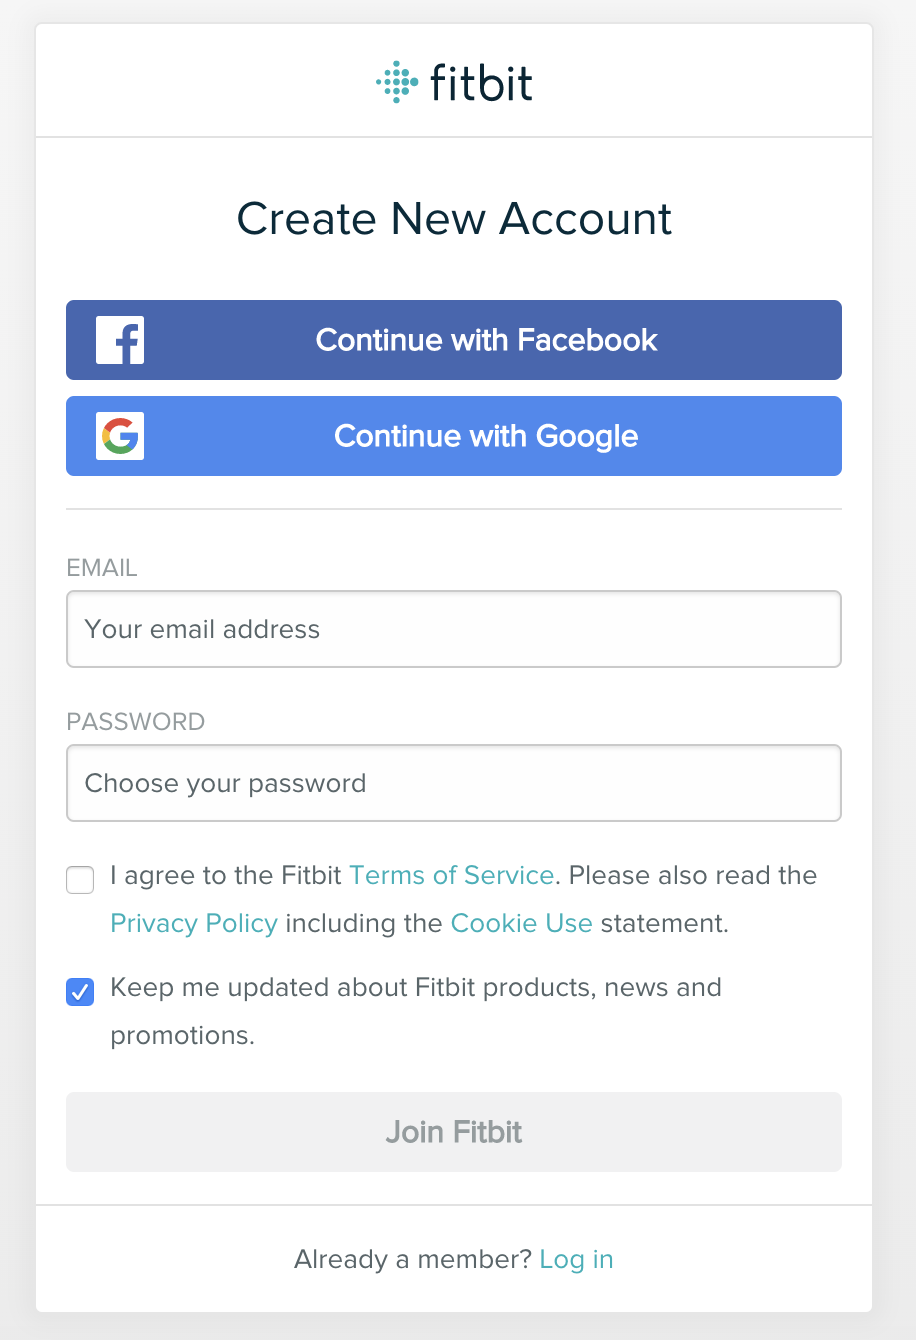
\includegraphics[width=0.40000\textwidth]{images/fitbitAccount.png}

After registering your Fitbit account, proceed to
\url{https://dev.fitbit.com/login} and login with the account
credentials you just created. Click on `manage' and `register an app' in
the navigation bar. You will then be presented with the screen show in
figure 2. Fill out the necessary registration fields and click
`register' at the bottom of the page.

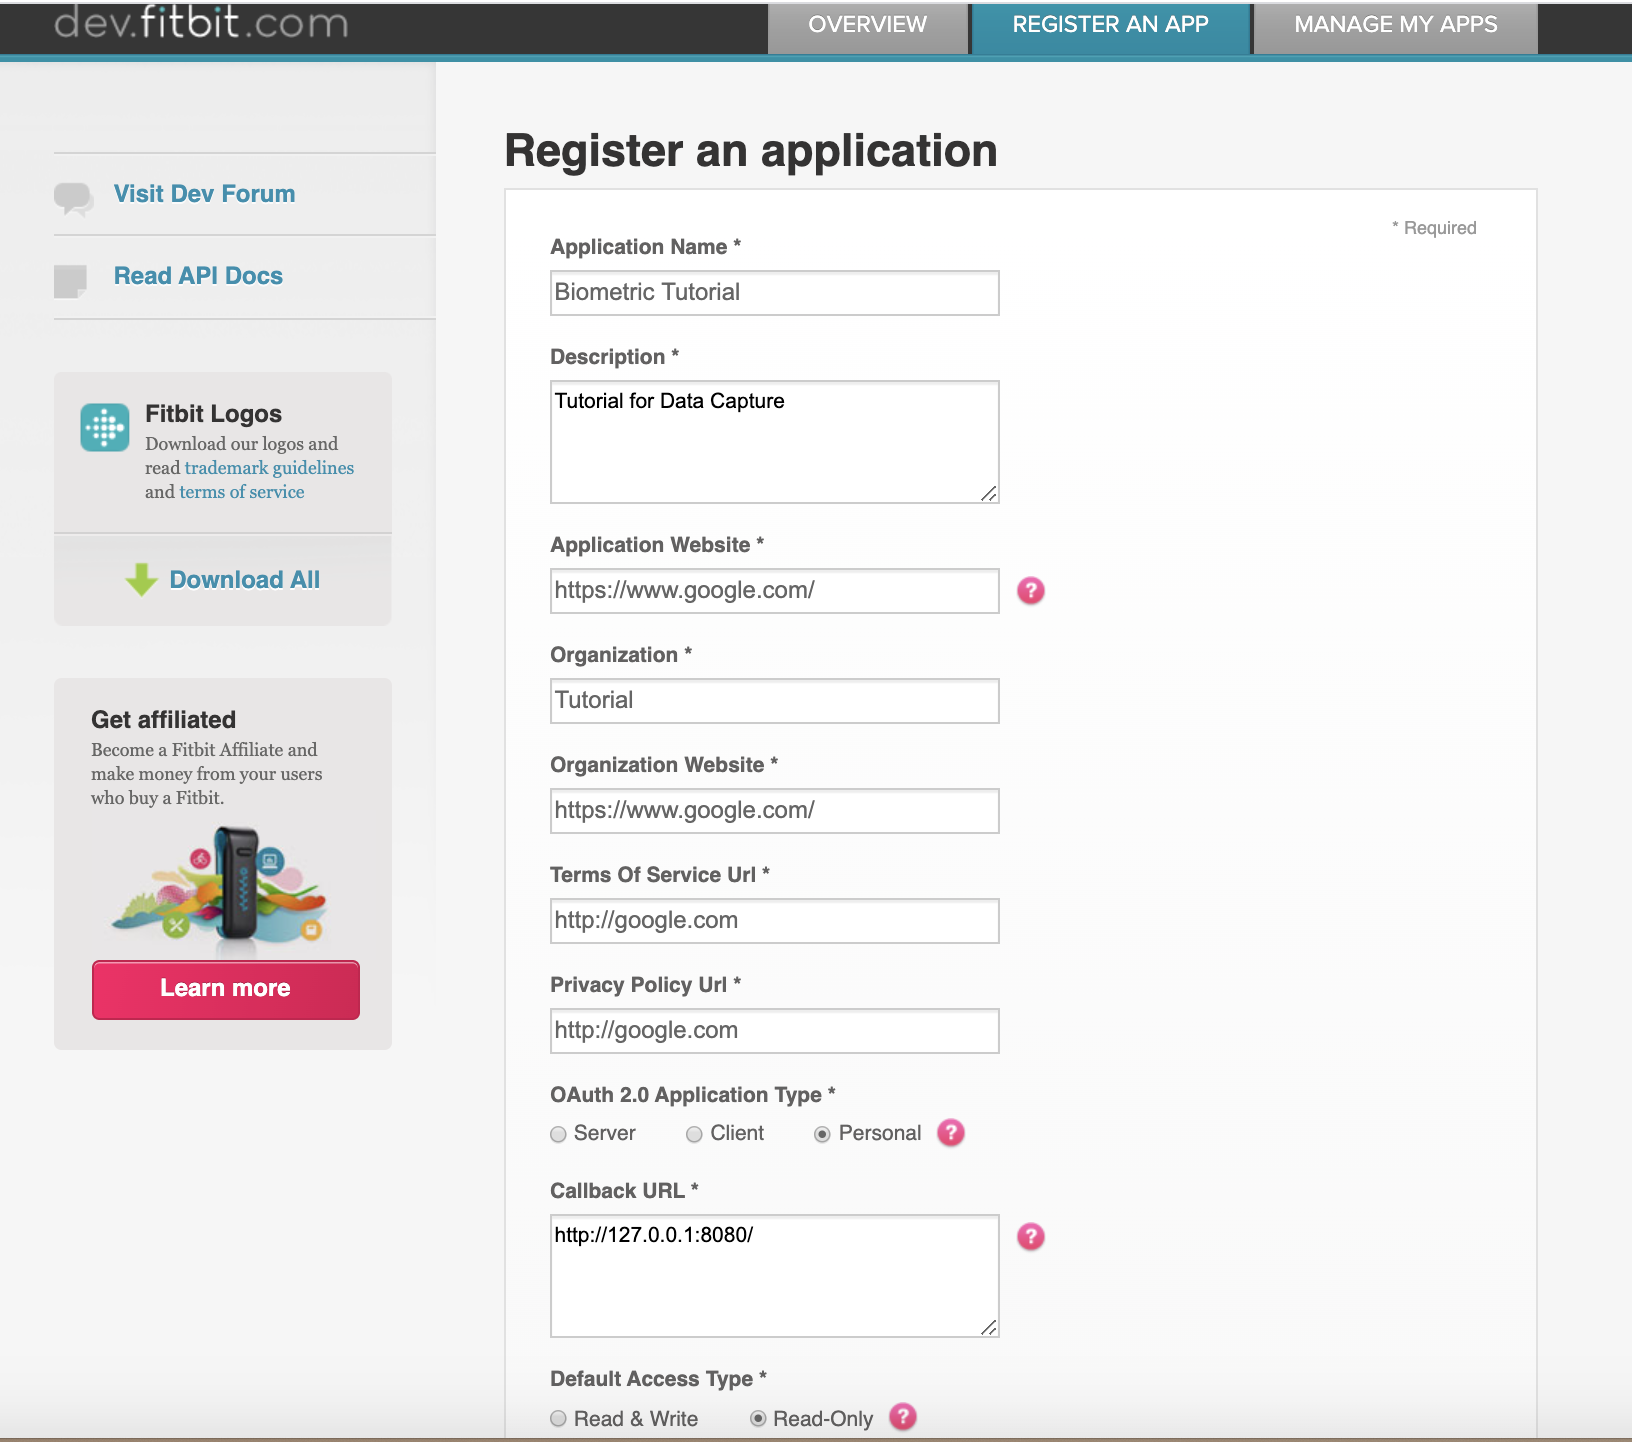
\includegraphics[width=0.75000\textwidth]{images/registerApp.png}

Now that an application is registered to your account, you can navigate
to your apps. When clicking on the recently created app you will see a
samilar display as in Figure 3.

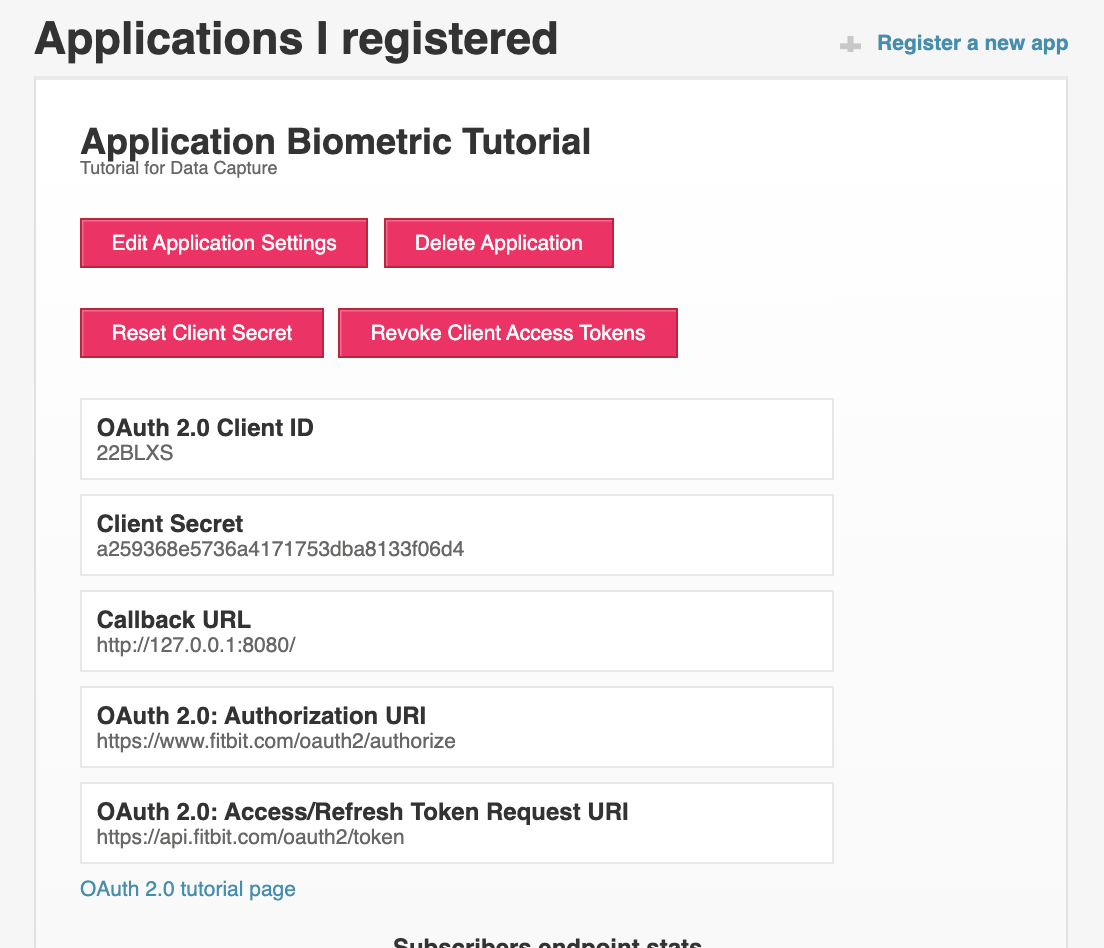
\includegraphics[width=0.75000\textwidth]{images/appDetails.png}

The creation and registration of this app with fitbit will be neccessary
for the entirity of the tutorial. We will return to the information
shown soon.

\chapter{Dependencies}\label{dependencies}

For this project, it will be easiest for work in an Anaconda
enirvonement. Anaconda is an open-source Data Science toolkit. It allows
users to easily work with thousands of open-source packages.

Install Anaconda here:
\url{https://docs.anaconda.com/anaconda/install/}. Follow the steps
provided to install for your machine.

After you have installed Anaconda, open the Anaconda Navigator. It will
look similar to the image below.

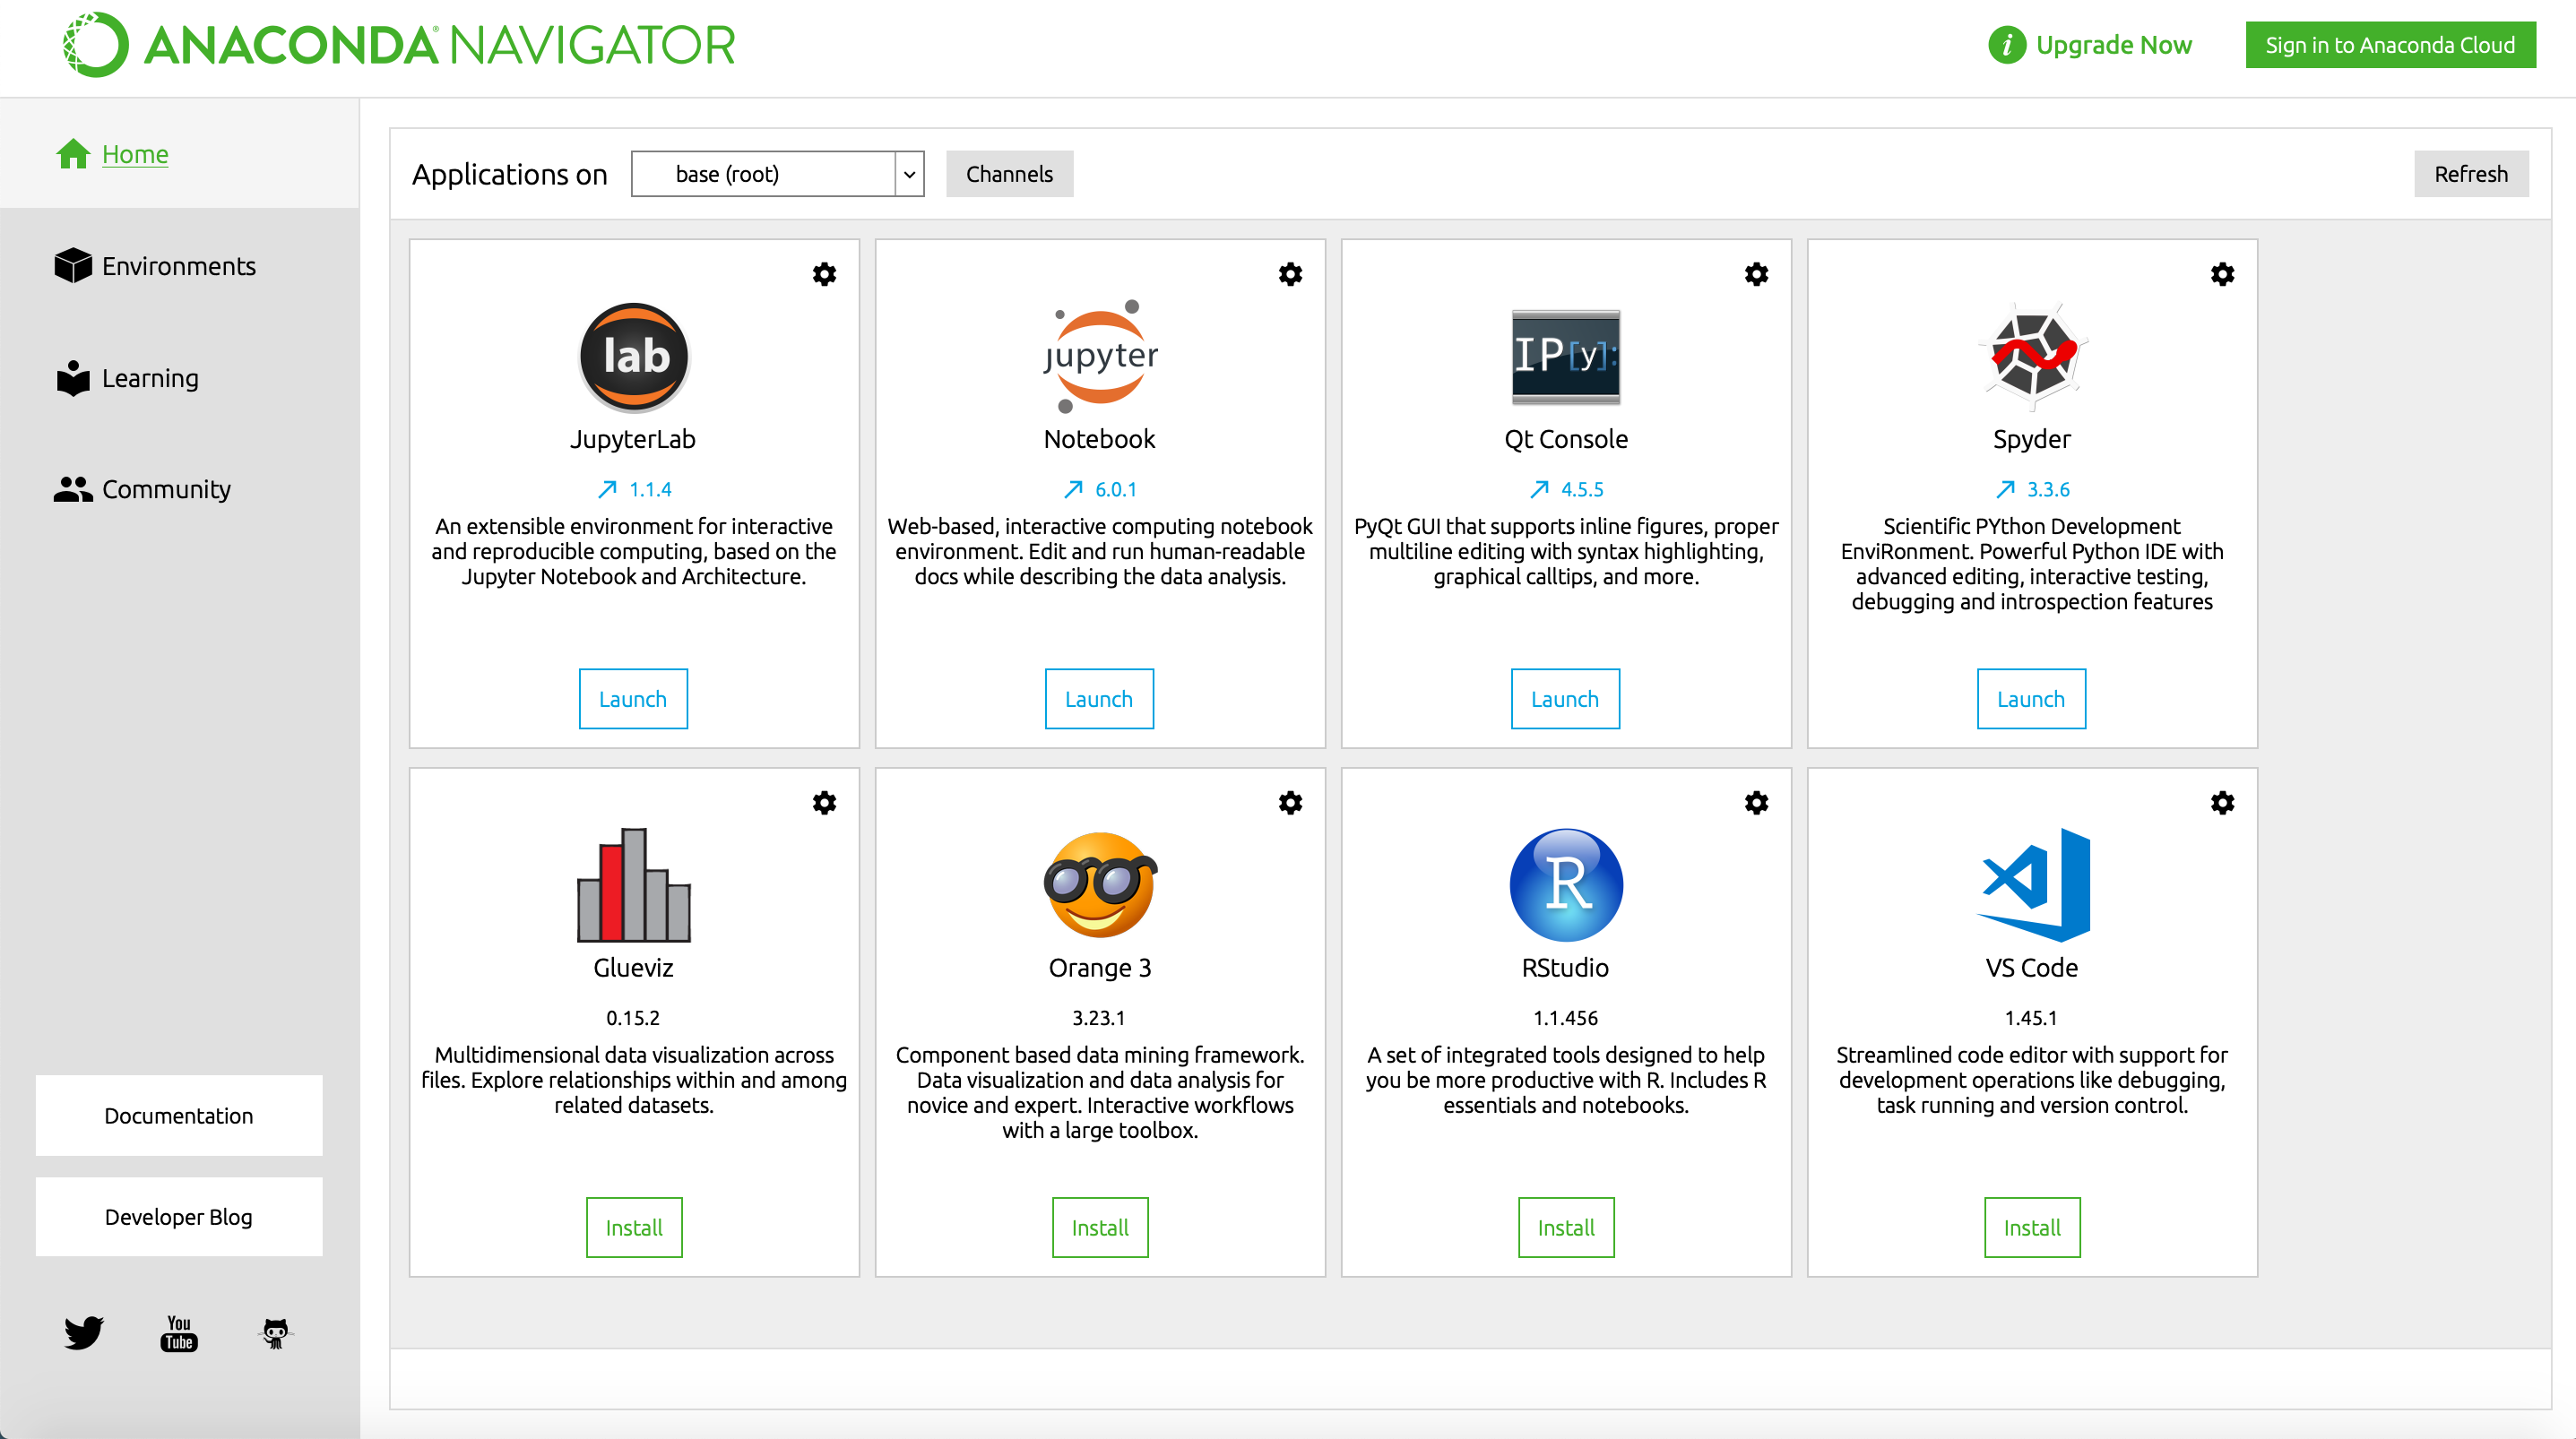
\includegraphics[width=0.80000\textwidth]{images/anacondanav.png}

On the left side navigation bar, click on evironments and then search
for `cherrypy'. Check the box next to cherrypy and click the green apply
button.

After, you be able to use the different applications offered through
anaconda. Jupyter notebook is great for writing programs in Python and
R.

\chapter{Working in Python}\label{working-in-python}

In this section, we will cover important computing fundamtentals using
the python programming language. These fundamentals are transferrable
between many programming languages so laying a strong foundation will
prove benfeficial.

\begin{longtable}[]{@{}l@{}}
\toprule
If you are new to python, it is in your best interest to review some of
the matieral at \url{https://www.w3schools.com/python/} for foundational
skills.\tabularnewline
\bottomrule
\end{longtable}

\section{Python Introduction}\label{python-introduction}

Python is an interpreted programming language that is known for its
simplicity, readability, and small learning curve. Python is one of the
most popular programming languages used today and learning to use Python
will provide fundamental computing skills.

For this tutorial, it is easiest to use a Jupyter Notebook. Create a new
notebook and select Python as the language. Before starting the
tutorial, add the follow imports at the top of your notebook:

\begin{Shaded}
\begin{Highlighting}[]
\CommentTok{# These are helpful packages that will aid our work through the tutorial!}
\ImportTok{import}\NormalTok{ sys}
\ImportTok{import}\NormalTok{ csv}
\ImportTok{import}\NormalTok{ requests}
\ImportTok{from}\NormalTok{ collections }\ImportTok{import}\NormalTok{ defaultdict}
\end{Highlighting}
\end{Shaded}

\section{Reading Data, Conditionals,
Loops}\label{reading-data-conditionals-loops}

The data for this tutorial can be found at
\url{https://raw.githubusercontent.com/fivethirtyeight/data/master/us-weather-history/KNYC.csv}.
The data is in CSV format meaning that each new value is seperated by a
comma. Take a look at the raw data by visiting the link. It is data on
weather patterns in NYC during parts of 2014 and 2015.

Now that we know the format of the data, lets read it into our Notebook.

\begin{Shaded}
\begin{Highlighting}[]
\CommentTok{# open the file directly from the link}
\BuiltInTok{file} \OperatorTok{=}\NormalTok{ requests.get(}\StringTok{"https://raw.githubusercontent.com/fivethirtyeight/data/master/us-weather-history/KNYC.csv"}\NormalTok{).text}
\end{Highlighting}
\end{Shaded}

Right now, the file is a string. To work with our data, we need to clean
it and get it to a format for better analysis. To start, we will need to
remove any unneccessary whitespace and create a list where each element
is a new line.

\begin{Shaded}
\begin{Highlighting}[]
\CommentTok{# strip() - method that removes whitespace }
\CommentTok{# split("\textbackslash{}n") - method that returns a list of values broken by input characters from the input string.}
\BuiltInTok{file} \OperatorTok{=} \BuiltInTok{file}\NormalTok{.strip().split(}\StringTok{'}\CharTok{\textbackslash{}n}\StringTok{'}\NormalTok{)}
\end{Highlighting}
\end{Shaded}

Our file is now a list, where each element is one row (run print(file)
if you would like to check). Our objective is to make each element of
the list, a new list! We can easily do this using a for loop. A for loop
will iterate over a sequence (i.e lists, dictionaries, tuples, sets) and
perform itertive commands in the loop. Lets try to clean our data some
more.

\begin{Shaded}
\begin{Highlighting}[]
\CommentTok{# for each element of the list, split the element by comma to make sublists}
\ControlFlowTok{for}\NormalTok{ row }\KeywordTok{in} \BuiltInTok{range}\NormalTok{(}\BuiltInTok{len}\NormalTok{(}\BuiltInTok{file}\NormalTok{)):}
    \BuiltInTok{file}\NormalTok{[row] }\OperatorTok{=} \BuiltInTok{file}\NormalTok{[row].split(}\StringTok{","}\NormalTok{)}
\end{Highlighting}
\end{Shaded}

Great, our data is cleaned! Let's view our file with a loop:

\begin{Shaded}
\begin{Highlighting}[]
\CommentTok{# Print the first five file lines of the data }
\ControlFlowTok{for}\NormalTok{ row }\KeywordTok{in} \BuiltInTok{file}\NormalTok{[}\DecValTok{0}\NormalTok{:}\DecValTok{5}\NormalTok{]: }
  \BuiltInTok{print}\NormalTok{(row)}
\end{Highlighting}
\end{Shaded}

\begin{verbatim}
## ['date', 'actual_mean_temp', 'actual_min_temp', 'actual_max_temp', 'average_min_temp', 'average_max_temp', 'record_min_temp', 'record_max_temp', 'record_min_temp_year', 'record_max_temp_year', 'actual_precipitation', 'average_precipitation', 'record_precipitation']
## ['2014-7-1', '81', '72', '89', '68', '83', '52', '100', '1943', '1901', '0.00', '0.12', '2.17']
## ['2014-7-2', '82', '72', '91', '68', '83', '56', '100', '2001', '1966', '0.96', '0.13', '1.79']
## ['2014-7-3', '78', '69', '87', '68', '83', '54', '103', '1933', '1966', '1.78', '0.12', '2.80']
## ['2014-7-4', '70', '65', '74', '68', '84', '55', '102', '1986', '1949', '0.14', '0.13', '1.76']
\end{verbatim}

Notice that the first line is the header line and the rest of the lines
are data for the corresponding headers. Let's take a look at the maximum
temperature on the first five days listed in the data set.

\begin{Shaded}
\begin{Highlighting}[]
\ControlFlowTok{for}\NormalTok{ row }\KeywordTok{in} \BuiltInTok{file}\NormalTok{[}\DecValTok{0}\NormalTok{:}\DecValTok{6}\NormalTok{]:}
  \BuiltInTok{print}\NormalTok{(}\StringTok{"}\SpecialCharTok{%-20s}\StringTok{ }\SpecialCharTok\NormalTok{ (row[}\DecValTok{0}\NormalTok{],row[}\DecValTok{3}\NormalTok{])) }\CommentTok{# simple string formatting techniques!}
\end{Highlighting}
\end{Shaded}

\begin{verbatim}
## date                 actual_max_temp
## 2014-7-1             89
## 2014-7-2             91
## 2014-7-3             87
## 2014-7-4             74
## 2014-7-5             81
\end{verbatim}

\section{Pandas and Numpy}\label{pandas-and-numpy}

While our data is already organized well, more complex analysis with
data in this format can get tedious. A popular data maniputlation and
analysis software is called Pandas. Let's explore the functionality of
Pandas!

To start, let's create the list of headers:

\begin{Shaded}
\begin{Highlighting}[]
\NormalTok{headers }\OperatorTok{=} \BuiltInTok{file}\NormalTok{[}\DecValTok{0}\NormalTok{]}
\NormalTok{headers}
\end{Highlighting}
\end{Shaded}

\begin{verbatim}
## ['date', 'actual_mean_temp', 'actual_min_temp', 'actual_max_temp', 'average_min_temp', 'average_max_temp', 'record_min_temp', 'record_max_temp', 'record_min_temp_year', 'record_max_temp_year', 'actual_precipitation', 'average_precipitation', 'record_precipitation']
\end{verbatim}

Next, we will reformat our original list of data so that the headers are
removed:

\begin{Shaded}
\begin{Highlighting}[]
\ImportTok{import}\NormalTok{ datetime}
\NormalTok{data }\OperatorTok{=} \BuiltInTok{file}\NormalTok{[}\DecValTok{1}\NormalTok{:]               }\CommentTok{# remove header}

\ControlFlowTok{for}\NormalTok{ row }\KeywordTok{in}\NormalTok{ data:              }\CommentTok{# convert data from strings to floats}
    \ControlFlowTok{for}\NormalTok{ i }\KeywordTok{in} \BuiltInTok{range}\NormalTok{(}\DecValTok{0}\NormalTok{,}\DecValTok{13}\NormalTok{):}
        \ControlFlowTok{if}\NormalTok{ i }\OperatorTok{==} \DecValTok{0}\NormalTok{:}
\NormalTok{            row[i]}\OperatorTok{=}\NormalTok{ datetime.datetime.strptime(row[i],}\StringTok{'%Y-%m-}\SpecialCharTok{%d}\StringTok{'}\NormalTok{)}
        \ControlFlowTok{else}\NormalTok{: }
\NormalTok{            row[i] }\OperatorTok{=} \BuiltInTok{float}\NormalTok{(row[i])}
\end{Highlighting}
\end{Shaded}

Lastly, we will place our data into a pandas dataframe:

\begin{Shaded}
\begin{Highlighting}[]
\ImportTok{import}\NormalTok{ pandas }\ImportTok{as}\NormalTok{ pd}
\NormalTok{df }\OperatorTok{=}\NormalTok{ pd.DataFrame(data, columns }\OperatorTok{=}\NormalTok{ headers)}
\NormalTok{df.head()     }\CommentTok{# .head() is a way to view the first 5 rows of the dataframe}
\end{Highlighting}
\end{Shaded}

\begin{verbatim}
##         date  actual_mean_temp  ...  average_precipitation  record_precipitation
## 0 2014-07-01              81.0  ...                   0.12                  2.17
## 1 2014-07-02              82.0  ...                   0.13                  1.79
## 2 2014-07-03              78.0  ...                   0.12                  2.80
## 3 2014-07-04              70.0  ...                   0.13                  1.76
## 4 2014-07-05              72.0  ...                   0.12                  3.07
## 
## [5 rows x 13 columns]
\end{verbatim}

Great! Now we can perfom analysis very easily on our data! For example,
we can find some very valuable statistics with one simple command!

\begin{Shaded}
\begin{Highlighting}[]
\NormalTok{df.describe()}
\end{Highlighting}
\end{Shaded}

\begin{verbatim}
##        actual_mean_temp  ...  record_precipitation
## count        365.000000  ...            365.000000
## mean          54.736986  ...              2.386137
## std           18.679979  ...              1.045702
## min           11.000000  ...              0.860000
## 25%           39.000000  ...              1.690000
## 50%           58.000000  ...              2.160000
## 75%           72.000000  ...              2.750000
## max           85.000000  ...              8.280000
## 
## [8 rows x 12 columns]
\end{verbatim}

Pandas is a very poweful tool! More about pandas can be learned at
\url{https://pandas.pydata.org/pandas-docs/version/0.25.3/}.

\section{Vizualizations with
Matplotlib}\label{vizualizations-with-matplotlib}

Lastly, we can make a simple vizualization of our data using another
package called Matplotlib. It is a plotting library for the python
programming langauge.

\begin{Shaded}
\begin{Highlighting}[]
\ImportTok{import}\NormalTok{ matplotlib.pyplot }\ImportTok{as}\NormalTok{ plt}
\NormalTok{fig, ax }\OperatorTok{=}\NormalTok{ plt.subplots(figsize}\OperatorTok{=}\NormalTok{(}\DecValTok{12}\NormalTok{, }\DecValTok{12}\NormalTok{))}
\NormalTok{y }\OperatorTok{=}\NormalTok{df[}\StringTok{'actual_max_temp'}\NormalTok{]}
\NormalTok{x}\OperatorTok{=}\NormalTok{df[}\StringTok{'date'}\NormalTok{]}
\NormalTok{ax.plot(x,y)}
\NormalTok{ax.}\BuiltInTok{set}\NormalTok{(xlabel}\OperatorTok{=}\StringTok{"Date"}\NormalTok{, ylabel}\OperatorTok{=}\StringTok{"Max Temp (F)"}\NormalTok{, title}\OperatorTok{=}\StringTok{"Max Temperarure in New York City"}\NormalTok{)}
\end{Highlighting}
\end{Shaded}

\begin{verbatim}
## [Text(0.5, 0, 'Date'), Text(0, 0.5, 'Max Temp (F)'), Text(0.5, 1.0, 'Max Temperarure in New York City')]
\end{verbatim}

\begin{Shaded}
\begin{Highlighting}[]
\NormalTok{plt.gcf().autofmt_xdate()}
\NormalTok{plt.show()}
\end{Highlighting}
\end{Shaded}

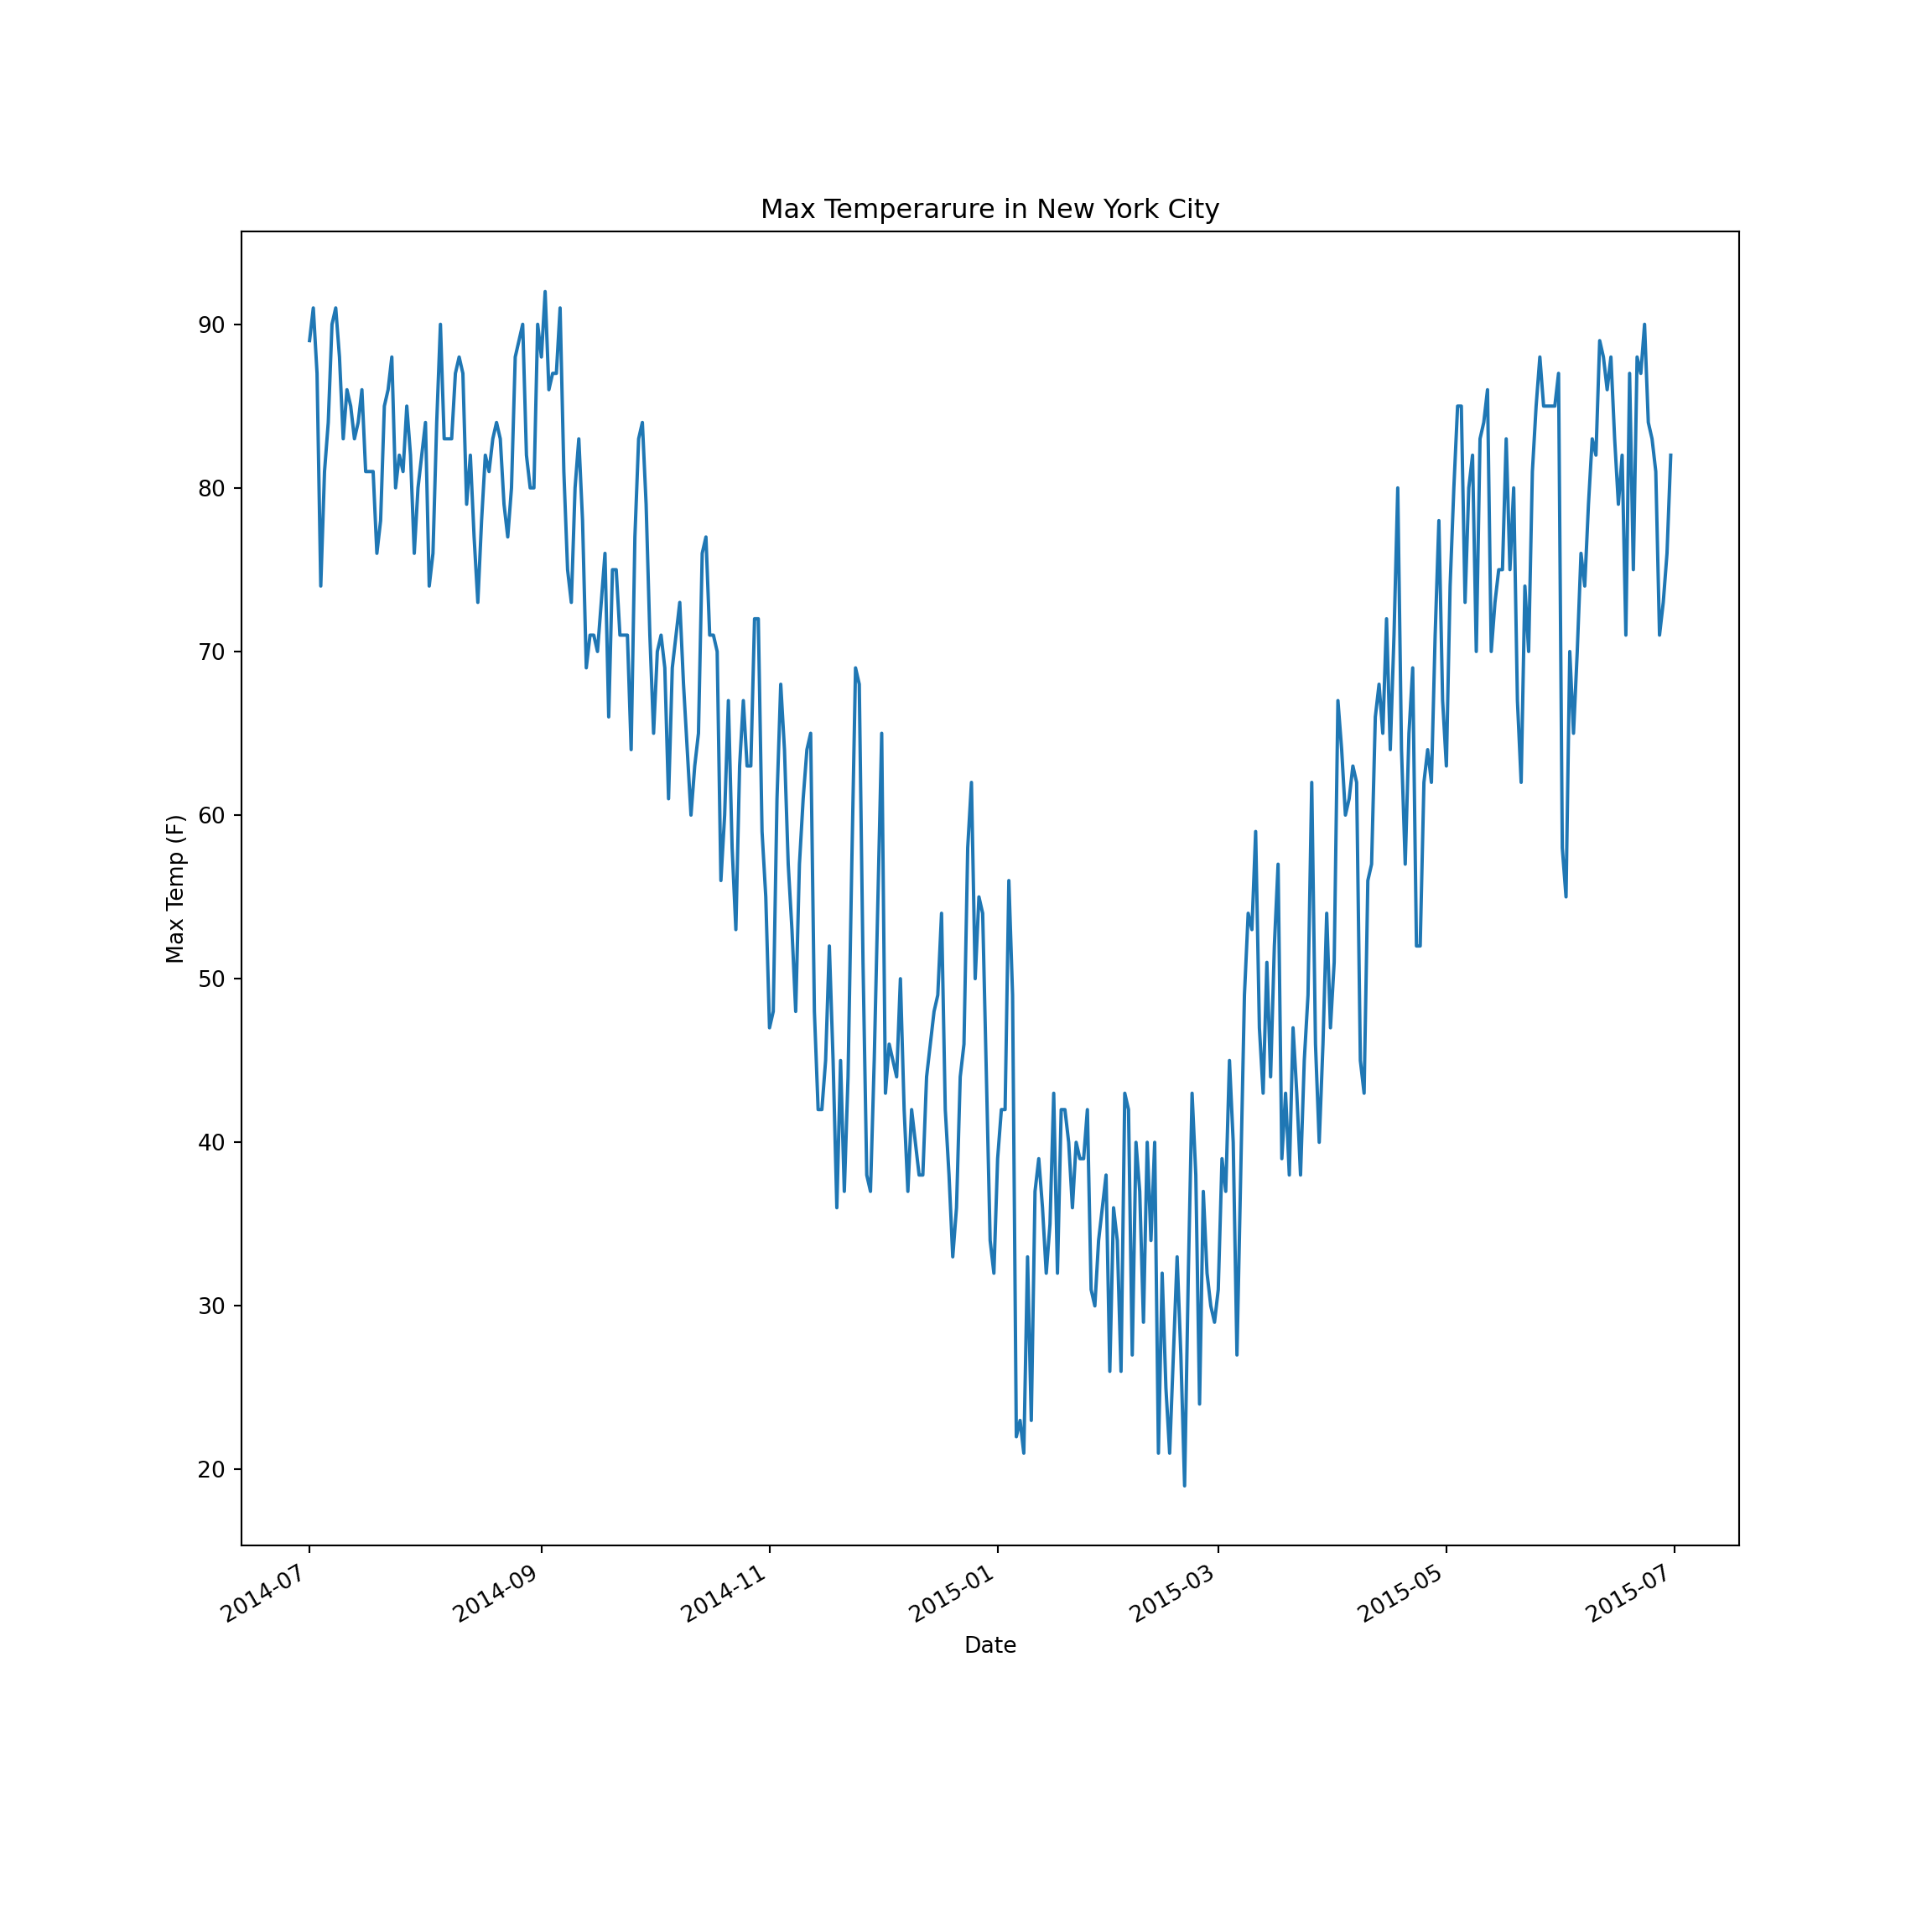
\includegraphics{bookdown-demo_files/figure-latex/unnamed-chunk-34-1.pdf}

Matplot has much more funtionality than this simple example. Refer to
the documentation at \url{https://matplotlib.org/3.2.1/contents.html}
for more information!

\chapter{Tutorial - Data Capture in
Python}\label{tutorial---data-capture-in-python}

\section{Getting Started}\label{getting-started}

Before starting this section of the tutorial, we need to download the
Fitbit API.

Navigate to \url{https://github.com/orcasgit/python-fitbit} and click
the green `clone or download' button. Then, click download zip, and open
the zip file in the same folder that you are using within Anaconda.

Next, download python on to your computer at
\url{https://www.python.org/downloads/}. Click on the yellow `download'
button, open the downloaded file, and follow the steps to install.

Lastly, open a new terminal, and run the following commands:

\begin{Shaded}
\begin{Highlighting}[]
\NormalTok{pip install cherrypy (you can also use the Anaconda navigator to install cherrypy)}

\NormalTok{pip install requests}\OperatorTok{-}\NormalTok{oauthlib  }
\end{Highlighting}
\end{Shaded}

\section{Imports}\label{imports}

This project requires multiple packages. If the steps in the previous
sections have been followed, these import statements should run
seamlessly.

\begin{Shaded}
\begin{Highlighting}[]
\CommentTok{#Import the necessary packages}
\ImportTok{import}\NormalTok{ fitbit}
\ImportTok{import}\NormalTok{ gather_keys_oauth2 }\ImportTok{as}\NormalTok{ Oauth2}
\ImportTok{import}\NormalTok{ pandas }\ImportTok{as}\NormalTok{ pd }
\ImportTok{import}\NormalTok{ datetime}
\ImportTok{import}\NormalTok{ json}
\end{Highlighting}
\end{Shaded}

\section{Authentication}\label{authentication}

Remembering back to the Fibit Technology section, we registered an app
on the Fitbit Development site that will allow us to access our account
data. When we completed the registration of the app, we were given a
client id and client secret. These codes are unique to each individual
app that is registered and are neccessary for the authentication
process.

Use the following code gain access to your account:

\begin{Shaded}
\begin{Highlighting}[]
\NormalTok{CLIENT_ID }\OperatorTok{=} \StringTok{'22BLXS'} \CommentTok{#ENTER CLIENT ID CODE HERE }
\NormalTok{CLIENT_SECRET }\OperatorTok{=} \StringTok{'a259368e5736a4171753dba8133f06d4'} \CommentTok{#ENTER CLIENT SECRET CODE HERE}

\NormalTok{server }\OperatorTok{=}\NormalTok{ Oauth2.OAuth2Server(CLIENT_ID, CLIENT_SECRET)}
\NormalTok{server.browser_authorize()}
\NormalTok{ACCESS_TOKEN }\OperatorTok{=} \BuiltInTok{str}\NormalTok{(server.fitbit.client.session.token[}\StringTok{'access_token'}\NormalTok{])}
\NormalTok{REFRESH_TOKEN }\OperatorTok{=} \BuiltInTok{str}\NormalTok{(server.fitbit.client.session.token[}\StringTok{'refresh_token'}\NormalTok{])}
\NormalTok{auth2_client }\OperatorTok{=}\NormalTok{ fitbit.Fitbit(CLIENT_ID, CLIENT_SECRET, oauth2}\OperatorTok{=}\VariableTok{True}\NormalTok{, access_token}\OperatorTok{=}\NormalTok{ACCESS_TOKEN,}
\NormalTok{refresh_token}\OperatorTok{=}\NormalTok{REFRESH_TOKEN)}
\end{Highlighting}
\end{Shaded}

When the code above is run for the first time, you will be directed to a
new browser with the following screen:

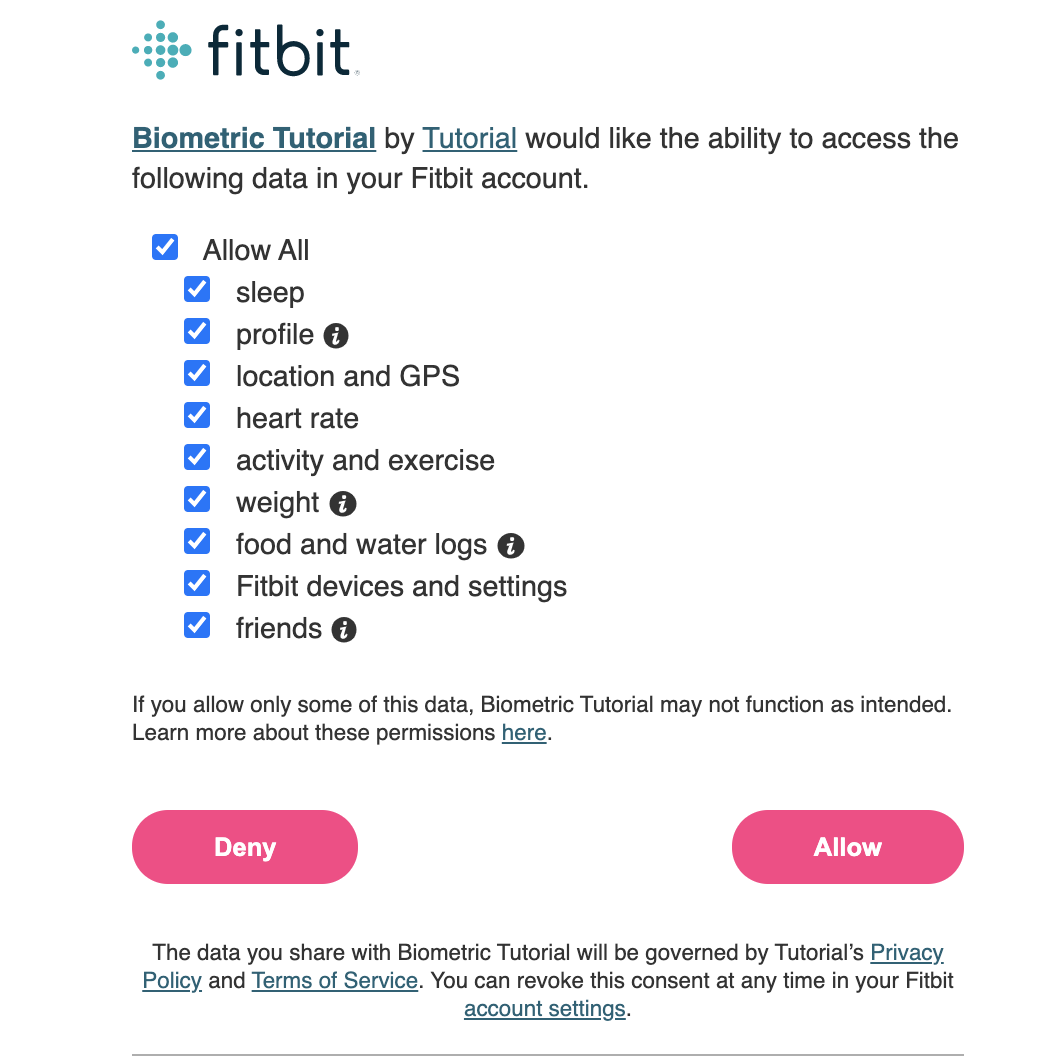
\includegraphics[width=0.80000\textwidth]{images/accessData.png}

Select `Allow All' and then `Allow'. Your browser will then display the
follow:

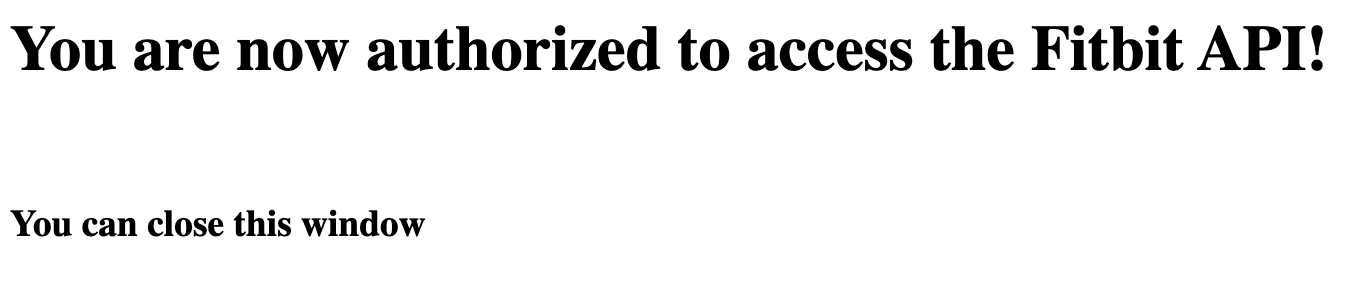
\includegraphics[width=0.80000\textwidth]{images/done.png}

When you have reached this screen, the authentication is complete and
you can now access your account data. According the fitbit
documentation, you can access your data, by default, for 8 hours until
you will have to reautheticate by running the authorization code above.

\section{Accessing Data}\label{accessing-data}

Now that the authentication is complete, we can access our data.

To start, we need to delcare a date to collect data from. Let's use
today's date:

\begin{Shaded}
\begin{Highlighting}[]
\NormalTok{today }\OperatorTok{=} \BuiltInTok{str}\NormalTok{(datetime.datetime.now().strftime(}\StringTok{"%Y-%m-}\SpecialCharTok{%d}\StringTok{"}\NormalTok{)) }\CommentTok{#todays date}
\end{Highlighting}
\end{Shaded}

Now we can view our `activities' data for todays date.

\begin{Shaded}
\begin{Highlighting}[]
\NormalTok{activities }\OperatorTok{=}\NormalTok{ auth2_client.activities(date }\OperatorTok{=}\NormalTok{ today)}
\end{Highlighting}
\end{Shaded}

Notice how the data is formatted in nested dictionary format, similar to
json file format. Becuase of this format, we need to decompose the
nested dictionaries to access our desired data.

For example, if we want to access the total distance traveled we can do
the following:

\begin{Shaded}
\begin{Highlighting}[]
\NormalTok{activities }\OperatorTok{=}\NormalTok{ auth2_client.activities(date }\OperatorTok{=}\NormalTok{ today)[}\StringTok{'summary'}\NormalTok{]}
\NormalTok{totalDistance }\OperatorTok{=}\NormalTok{ activities[}\StringTok{'distances'}\NormalTok{][}\DecValTok{0}\NormalTok{][}\StringTok{'distance'}\NormalTok{]}
\end{Highlighting}
\end{Shaded}

To access today's steps:

\begin{Shaded}
\begin{Highlighting}[]
\NormalTok{steps }\OperatorTok{=}\NormalTok{ activities[}\StringTok{'steps'}\NormalTok{]}
\end{Highlighting}
\end{Shaded}

The process is almost identical for accessing other types of data
(i.e.~sleep, heart, and weight data).

\section{Processing Data}\label{processing-data}

Because we are now familiar with the structure of of data, we can begin
processing it!

To collect activities data:

\begin{Shaded}
\begin{Highlighting}[]
\CommentTok{#gets all Activities Data}
\KeywordTok{def}\NormalTok{ getActivities(myDate): }
\NormalTok{    activities }\OperatorTok{=}\NormalTok{ auth2_client.activities(date }\OperatorTok{=}\NormalTok{ myDate)[}\StringTok{'summary'}\NormalTok{]}

\NormalTok{    totalDistance }\OperatorTok{=}\NormalTok{ activities[}\StringTok{'distances'}\NormalTok{][}\DecValTok{0}\NormalTok{][}\StringTok{'distance'}\NormalTok{]}
\NormalTok{    veryActiveDistance }\OperatorTok{=}\NormalTok{ activities[}\StringTok{'distances'}\NormalTok{][}\DecValTok{3}\NormalTok{][}\StringTok{'distance'}\NormalTok{]}
\NormalTok{    moderatleyActiveDistance }\OperatorTok{=}\NormalTok{ activities[}\StringTok{'distances'}\NormalTok{][}\DecValTok{4}\NormalTok{][}\StringTok{'distance'}\NormalTok{]}
\NormalTok{    lightlyActiveDistance }\OperatorTok{=}\NormalTok{ activities[}\StringTok{'distances'}\NormalTok{][}\DecValTok{5}\NormalTok{][}\StringTok{'distance'}\NormalTok{]}
\NormalTok{    veryActiveMinutes }\OperatorTok{=}\NormalTok{ activities[}\StringTok{'veryActiveMinutes'}\NormalTok{]}
\NormalTok{    fairlyActiveMinutes }\OperatorTok{=}\NormalTok{ activities[}\StringTok{'fairlyActiveMinutes'}\NormalTok{]}
\NormalTok{    lightlyActiveMinutes }\OperatorTok{=}\NormalTok{ activities[}\StringTok{'lightlyActiveMinutes'}\NormalTok{]}
\NormalTok{    sedentaryMinutes }\OperatorTok{=}\NormalTok{ activities[}\StringTok{'sedentaryMinutes'}\NormalTok{]}
\NormalTok{    floorsClimbed }\OperatorTok{=}\NormalTok{ activities[}\StringTok{'floors'}\NormalTok{]}
\NormalTok{    daySteps }\OperatorTok{=}\NormalTok{activities[}\StringTok{'steps'}\NormalTok{]}
    
    \ControlFlowTok{return}\NormalTok{ totalDistance, veryActiveDistance, moderatleyActiveDistance, lightlyActiveDistance,   veryActiveMinutes, fairlyActiveMinutes, lightlyActiveMinutes, sedentaryMinutes, floorsClimbed, daySteps}
\end{Highlighting}
\end{Shaded}

To collect sleep data:

\begin{Shaded}
\begin{Highlighting}[]
\CommentTok{#gets all Sleep data}
\KeywordTok{def}\NormalTok{ getSleep(myDate): }
\NormalTok{    nightSleep }\OperatorTok{=}\NormalTok{ auth2_client.sleep(date }\OperatorTok{=}\NormalTok{ myDate)[}\StringTok{'sleep'}\NormalTok{]}
    
\NormalTok{    sleepEfficiency }\OperatorTok{=} \VariableTok{None}
\NormalTok{    minutesAsleep }\OperatorTok{=} \VariableTok{None}
    
    \ControlFlowTok{if} \BuiltInTok{len}\NormalTok{(nightSleep) }\OperatorTok{!=} \DecValTok{0}\NormalTok{:}
\NormalTok{        sleepEfficiency }\OperatorTok{=}\NormalTok{ nightSleep[}\DecValTok{0}\NormalTok{][}\StringTok{'efficiency'}\NormalTok{]}
\NormalTok{        minutesAsleep }\OperatorTok{=}\NormalTok{ nightSleep[}\DecValTok{0}\NormalTok{][}\StringTok{'minutesAsleep'}\NormalTok{]}
        
    \ControlFlowTok{return}\NormalTok{ sleepEfficiency, minutesAsleep}
\end{Highlighting}
\end{Shaded}

To collect heart data:

\begin{Shaded}
\begin{Highlighting}[]
\CommentTok{#gets all Heart Data}
\KeywordTok{def}\NormalTok{ getHeart(myDate): }
\NormalTok{        heartRates }\OperatorTok{=}\NormalTok{ auth2_client.intraday_time_series(}\StringTok{'activities/heart'}\NormalTok{, base_date}\OperatorTok{=}\NormalTok{myDate, detail_level}\OperatorTok{=}\StringTok{'1sec'}\NormalTok{)[}\StringTok{'activities-heart'}\NormalTok{][}\DecValTok{0}\NormalTok{][}\StringTok{'value'}\NormalTok{]}

\NormalTok{        HRrange30to100 }\OperatorTok{=} \VariableTok{None}
\NormalTok{        HRrange100to140 }\OperatorTok{=} \VariableTok{None}
\NormalTok{        HRrange140to170 }\OperatorTok{=} \VariableTok{None}
\NormalTok{        HRrange170to220 }\OperatorTok{=} \VariableTok{None}
\NormalTok{        avgRestingHR }\OperatorTok{=} \VariableTok{None}
        
        \ControlFlowTok{if} \BuiltInTok{len}\NormalTok{(heartRates) }\OperatorTok{==} \DecValTok{3}\NormalTok{:}
\NormalTok{            HRrange30to100 }\OperatorTok{=}\NormalTok{ heartRates[}\StringTok{'heartRateZones'}\NormalTok{][}\DecValTok{0}\NormalTok{][}\StringTok{'minutes'}\NormalTok{]}
\NormalTok{            HRrange100to140 }\OperatorTok{=}\NormalTok{ heartRates[}\StringTok{'heartRateZones'}\NormalTok{][}\DecValTok{1}\NormalTok{][}\StringTok{'minutes'}\NormalTok{]}
\NormalTok{            HRrange140to170 }\OperatorTok{=}\NormalTok{ heartRates[}\StringTok{'heartRateZones'}\NormalTok{][}\DecValTok{2}\NormalTok{][}\StringTok{'minutes'}\NormalTok{]}
\NormalTok{            HRrange170to220 }\OperatorTok{=}\NormalTok{ heartRates[}\StringTok{'heartRateZones'}\NormalTok{][}\DecValTok{3}\NormalTok{][}\StringTok{'minutes'}\NormalTok{]}
\NormalTok{            avgRestingHR }\OperatorTok{=}\NormalTok{ heartRates[}\StringTok{'restingHeartRate'}\NormalTok{]}
            
        \ControlFlowTok{return}\NormalTok{ HRrange30to100, HRrange100to140, HRrange140to170, HRrange170to220, avgRestingHR}
\end{Highlighting}
\end{Shaded}

To collect weight data:

\begin{Shaded}
\begin{Highlighting}[]
\CommentTok{#gets all Weight Data}
\KeywordTok{def}\NormalTok{ getWeight(myDate):}
\NormalTok{    grabWeight }\OperatorTok{=}\NormalTok{ auth2_client.get_bodyweight(base_date }\OperatorTok{=}\NormalTok{ myDate)[}\StringTok{'weight'}\NormalTok{]}
\NormalTok{    weight }\OperatorTok{=} \VariableTok{None}
\NormalTok{    BMI }\OperatorTok{=} \VariableTok{None}
    \ControlFlowTok{if} \BuiltInTok{len}\NormalTok{(grabWeight) }\OperatorTok{>} \DecValTok{0}\NormalTok{:}
\NormalTok{        weight }\OperatorTok{=}\NormalTok{ grabWeight[}\DecValTok{0}\NormalTok{][}\StringTok{'weight'}\NormalTok{]}
\NormalTok{        BMI }\OperatorTok{=}\NormalTok{ grabWeight[}\DecValTok{0}\NormalTok{][}\StringTok{'bmi'}\NormalTok{]}
        
    \ControlFlowTok{return}\NormalTok{ weight, BMI}
\end{Highlighting}
\end{Shaded}

Now that we have the functions to capture the data, we can process our
data with a pandas data frame:

\begin{Shaded}
\begin{Highlighting}[]
\CommentTok{#creates empty data frame}
\NormalTok{biometricDF }\OperatorTok{=}\NormalTok{ pd.DataFrame(columns}\OperatorTok{=}\NormalTok{[}\StringTok{"Date"}\NormalTok{, }\StringTok{"Steps"}\NormalTok{, }\StringTok{"Floors Climbed"}\NormalTok{, }\StringTok{"Total Miles"}\NormalTok{, }\StringTok{"Lightly Active Miles"}\NormalTok{, }
                                    \StringTok{"Moderately Active Miles"}\NormalTok{, }\StringTok{"Very Active Miles"}\NormalTok{, }\StringTok{"Sedentary Minutes"}\NormalTok{, }
                                    \StringTok{"Lightly Active Minutes"}\NormalTok{, }\StringTok{"Fairly Active Minutes"}\NormalTok{, }\StringTok{"Very Active Minutes"}\NormalTok{, }
                                    \StringTok{"HR 30-100 Minutes"}\NormalTok{, }\StringTok{"HR 100-140 Minutes"}\NormalTok{, }\StringTok{"HR 140-170 Minutes"}\NormalTok{, }
                                    \StringTok{"HR 170-220 Minutes"}\NormalTok{, }\StringTok{"Average Resting HR"}\NormalTok{])}
\end{Highlighting}
\end{Shaded}

Next, we will need a function to collect all the data togother and place
it into a data frame:

\begin{Shaded}
\begin{Highlighting}[]
\CommentTok{#adds data to data frame}
\KeywordTok{def}\NormalTok{ getBiometricData(myDF, myDate):}
\NormalTok{    totalDistance, veryActiveDistance, moderatleyActiveDistance, lightlyActiveDistance, veryActiveMinutes, fairlyActiveMinutes, lightlyActiveMinutes, sedentaryMinutes, floorsClimbed, daySteps }\OperatorTok{=}\NormalTok{ getActivities(myDate)}
    
\NormalTok{    sleepEfficiency, minutesAsleep }\OperatorTok{=}\NormalTok{ getSleep(myDate)}
    
\NormalTok{    HRrange30to100, HRrange100to140, HRrange140to170, HRrange170to220, avgRestingHR }\OperatorTok{=}\NormalTok{ getHeart(myDate)}
\NormalTok{    weight, BMI }\OperatorTok{=}\NormalTok{ getWeight(myDate)}
    
\NormalTok{    todaysData }\OperatorTok{=}\NormalTok{ \{}\StringTok{"Date"}\NormalTok{ : myDate, }\StringTok{"Steps"}\NormalTok{ : daySteps, }\StringTok{"Floors Climbed"}\NormalTok{ : floorsClimbed, }\StringTok{"Total Miles"}\NormalTok{: totalDistance, }\StringTok{"Lightly Active Miles"}\NormalTok{: lightlyActiveDistance, }\StringTok{"Moderately Active Miles"}\NormalTok{ : moderatleyActiveDistance, }\StringTok{"Very Active Miles"}\NormalTok{ : veryActiveDistance, }\StringTok{"Sedentary Minutes"}\NormalTok{: sedentaryMinutes, }\StringTok{"Lightly Active Minutes"}\NormalTok{: lightlyActiveMinutes, }\StringTok{"Fairly Active Minutes"}\NormalTok{ : fairlyActiveMinutes, }\StringTok{"Very Active Minutes"}\NormalTok{ : veryActiveMinutes,}\StringTok{"HR 30-100 Minutes"}\NormalTok{ : HRrange30to100, }\StringTok{"HR 100-140 Minutes"}\NormalTok{: HRrange100to140, }\StringTok{"HR 140-170 Minutes"}\NormalTok{ : HRrange140to170, }\StringTok{"HR 170-220 Minutes"}\NormalTok{ : HRrange170to220, }\StringTok{"Average Resting HR"}\NormalTok{: avgRestingHR, }\StringTok{"Sleep Efficiency"}\NormalTok{ : sleepEfficiency, }\StringTok{"Weight"}\NormalTok{ : weight, }\StringTok{"Minutes Alseep"}\NormalTok{ : minutesAsleep, }\StringTok{"BMI"}\NormalTok{ : BMI\}}

\NormalTok{    biometricDF }\OperatorTok{=}\NormalTok{ myDF.append(todaysData, ignore_index}\OperatorTok{=}\VariableTok{True}\NormalTok{)}

    \ControlFlowTok{return}\NormalTok{ biometricDF}
\end{Highlighting}
\end{Shaded}

And, finally, creating the database with todays data:

\begin{Shaded}
\begin{Highlighting}[]
\NormalTok{biometricDF }\OperatorTok{=}\NormalTok{ getBiometricData(biometricDF, today) }\CommentTok{#append to data frame}
\end{Highlighting}
\end{Shaded}

\section{Storing Data}\label{storing-data}

This process can be replicated each day so data must be stored
appropriately. To start, we can export our data frame to a csv file and
save the files to a directory like this (I created a new folder named
bioDates to store all my Data):

\begin{Shaded}
\begin{Highlighting}[]
\NormalTok{biometricDF.to_csv(}\StringTok{'./bioDates/'} \OperatorTok{+}\NormalTok{ today }\OperatorTok{+} \StringTok{'.csv'}\NormalTok{)}
\end{Highlighting}
\end{Shaded}

In the following chapters of this tutorial, we will learn how to
concatenate the indiviudal daily csv files into one master file as well
as storing the data into a a SQL database!

\chapter{Working in Bash}\label{working-in-bash}

\section{Introduction}\label{introduction}

Unix is simply a computer operating operating system.

Bash, on the other hand, is a shell. Shells are command line interfaces
where where you can communcate with the computer via certain commands.
Lets explore some commands. Feel free to test these on your machine in a
terminal.

\subsection{Basic Commands}\label{basic-commands}

\subsubsection{pwd}\label{pwd}

The command `pwd' will display the current working directory.
Directories are file systems that contain references to other
durectories and files.

\subsubsection{ls}\label{ls}

In order to view the files contained within the directory, we can use
the command `ls'. This will list the files and sub-directories in the
current worrking directory

\subsubsection{cd}\label{cd}

`cd' stands for change directory and will change the working directory
to a specified directory using a file path. By just entering cd, you
will directed to your home directory

\subsubsection{mkdir}\label{mkdir}

With the `mkdir' command, a new directory will be created with the name
we provide within the current working directory.

\subsubsection{touch and nano}\label{touch-and-nano}

The `touch' command will create a new file within the current working
directory.

Heres and example

\begin{Shaded}
\begin{Highlighting}[]
\BuiltInTok{pwd}
\FunctionTok{mkdir}\NormalTok{ Example}
\BuiltInTok{cd}\NormalTok{ Example/}
\BuiltInTok{pwd}
\FunctionTok{touch}\NormalTok{ exampleTextFile.txt}
\FunctionTok{ls}
\end{Highlighting}
\end{Shaded}

\begin{verbatim}
## /home/runner/work/wearables-book/wearables-book
## mkdir: cannot create directory ‘Example’: File exists
## /home/runner/work/wearables-book/wearables-book/Example
## exampleTextFile.txt
\end{verbatim}

For more basic bash commands, refer to
\url{https://www.educative.io/blog/bash-shell-command-cheat-sheet}!

\section{Working with Data using
Bash}\label{working-with-data-using-bash}

Bash is very powerful when working with data. Let's explore an example
of some data analysis using bash commands.

First, we will retrieve some data using the `wget' command. This command
will dowload data from a URL and save it to the current durectory.

\begin{longtable}[]{@{}l@{}}
\toprule
\begin{minipage}[t]{0.03\columnwidth}\raggedright\strut
For Mac users:\strut
\end{minipage}\tabularnewline
\begin{minipage}[t]{0.03\columnwidth}\raggedright\strut
If the wget command returns the error `wget: command not found', then
run\strut
\end{minipage}\tabularnewline
\begin{minipage}[t]{0.03\columnwidth}\raggedright\strut
ruby -e ``\$(curl -fsSL
\url{https://raw.githubusercontent.com/Homebrew/install/master/install})''\strut
\end{minipage}\tabularnewline
\begin{minipage}[t]{0.03\columnwidth}\raggedright\strut
followed by\strut
\end{minipage}\tabularnewline
\begin{minipage}[t]{0.03\columnwidth}\raggedright\strut
brew install wget\strut
\end{minipage}\tabularnewline
\begin{minipage}[t]{0.03\columnwidth}\raggedright\strut
This process installs Homebrew, which is a package manager for missing
packages on macOS.\strut
\end{minipage}\tabularnewline
\bottomrule
\end{longtable}

\begin{Shaded}
\begin{Highlighting}[]
\FunctionTok{wget}\NormalTok{ https://raw.githubusercontent.com/fivethirtyeight/data/master/us-weather-history/KNYC.csv}
\end{Highlighting}
\end{Shaded}

\begin{verbatim}
## --2020-07-28 16:59:10--  https://raw.githubusercontent.com/fivethirtyeight/data/master/us-weather-history/KNYC.csv
## Resolving raw.githubusercontent.com (raw.githubusercontent.com)... 151.101.208.133
## Connecting to raw.githubusercontent.com (raw.githubusercontent.com)|151.101.208.133|:443... connected.
## HTTP request sent, awaiting response... 200 OK
## Length: 20604 (20K) [text/plain]
## Saving to: ‘KNYC.csv.5’
## 
##      0K .......... ..........                                 100% 2.64M=0.007s
## 
## 2020-07-28 16:59:10 (2.64 MB/s) - ‘KNYC.csv.5’ saved [20604/20604]
\end{verbatim}

Now, we can view the first n rows of the data. In this example, we will
view the first five lines

\begin{Shaded}
\begin{Highlighting}[]
\FunctionTok{head}\NormalTok{ -n5 KNYC.csv}
\end{Highlighting}
\end{Shaded}

\begin{verbatim}
## date,actual_mean_temp,actual_min_temp,actual_max_temp,average_min_temp,average_max_temp,record_min_temp,record_max_temp,record_min_temp_year,record_max_temp_year,actual_precipitation,average_precipitation,record_precipitation
## 2014-7-1,81,72,89,68,83,52,100,1943,1901,0.00,0.12,2.17
## 2014-7-2,82,72,91,68,83,56,100,2001,1966,0.96,0.13,1.79
## 2014-7-3,78,69,87,68,83,54,103,1933,1966,1.78,0.12,2.80
## 2014-7-4,70,65,74,68,84,55,102,1986,1949,0.14,0.13,1.76
\end{verbatim}

Another helpful way to view data is to save subsets of data to seperate
files.

Here we save the first 10 lines to a new file called short.csv.

\begin{Shaded}
\begin{Highlighting}[]
\FunctionTok{head}\NormalTok{ -n10 KNYC.csv }\OperatorTok{>}\NormalTok{short.csv}
\end{Highlighting}
\end{Shaded}

Now we can view the whole file using the `cat' command.

\begin{Shaded}
\begin{Highlighting}[]
\FunctionTok{cat}\NormalTok{ short.csv}
\end{Highlighting}
\end{Shaded}

\begin{verbatim}
## date,actual_mean_temp,actual_min_temp,actual_max_temp,average_min_temp,average_max_temp,record_min_temp,record_max_temp,record_min_temp_year,record_max_temp_year,actual_precipitation,average_precipitation,record_precipitation
## 2014-7-1,81,72,89,68,83,52,100,1943,1901,0.00,0.12,2.17
## 2014-7-2,82,72,91,68,83,56,100,2001,1966,0.96,0.13,1.79
## 2014-7-3,78,69,87,68,83,54,103,1933,1966,1.78,0.12,2.80
## 2014-7-4,70,65,74,68,84,55,102,1986,1949,0.14,0.13,1.76
## 2014-7-5,72,63,81,68,84,53,101,1979,1999,0.00,0.12,3.07
## 2014-7-6,75,66,84,68,84,54,103,1979,2010,0.00,0.13,1.97
## 2014-7-7,81,72,90,68,84,56,100,1914,2010,0.04,0.13,3.13
## 2014-7-8,81,71,91,69,84,56,100,1894,1993,0.39,0.14,1.80
## 2014-7-9,80,71,88,69,84,54,106,1963,1936,0.09,0.14,1.09
\end{verbatim}

We can also view specifc columns from our data using `cut'.

\begin{Shaded}
\begin{Highlighting}[]
\FunctionTok{cut}\NormalTok{ -d, -f1,4 short.csv}
\end{Highlighting}
\end{Shaded}

\begin{verbatim}
## date,actual_max_temp
## 2014-7-1,89
## 2014-7-2,91
## 2014-7-3,87
## 2014-7-4,74
## 2014-7-5,81
## 2014-7-6,84
## 2014-7-7,90
## 2014-7-8,91
## 2014-7-9,88
\end{verbatim}

Next, lets look at a specific row by using the `grep' command to search
by date.

\begin{Shaded}
\begin{Highlighting}[]
\FunctionTok{grep}\NormalTok{ 2015-2-23 KNYC.csv}
\end{Highlighting}
\end{Shaded}

\begin{verbatim}
## 2015-2-23,23,8,38,30,43,5,70,1889,1985,0.00,0.12,1.38
\end{verbatim}

\section{Bash Scripts}\label{bash-scripts}

Now that we have covered some of the basics of bash, let's explore a
powerful tool within bash called bash scripting. Writing bash srcipts is
similar to any other program where each new line is a command with an
intent to build upon previous computations.

We can create files that will perform the tasks within. Consider this:

If we want to write some bash commands that will write the time of day
to a file we can do something like

\begin{Shaded}
\begin{Highlighting}[]
\FunctionTok{touch}\NormalTok{ myDateFile.txt}
\FunctionTok{date} \OperatorTok{>>}\NormalTok{myDateFile.txt}
\end{Highlighting}
\end{Shaded}

running these commands each time we would like to write the date to the
.txt file would begin to be tedius after time. Bash scripts provide an
easy solution!

First, we will create a new .sh file.

\begin{Shaded}
\begin{Highlighting}[]
\FunctionTok{touch}\NormalTok{ myDateBash.sh}
\end{Highlighting}
\end{Shaded}

Then, using a text editor, we can edit the file and enter our code to
write the date to myDateFile.txt.

Paste the following command into a terminal (be sure your working
directory is the same directory as where you saved your bash file):

vi myDateBash.sh

You will be presented with a screen that looks like the following image.

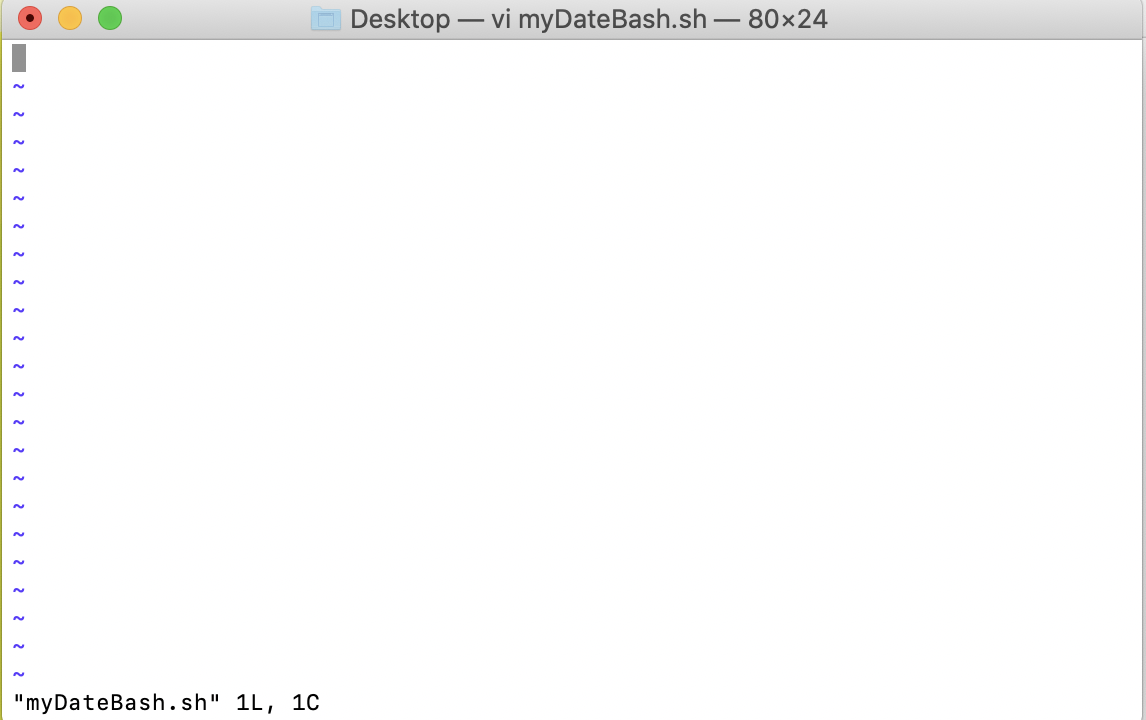
\includegraphics[width=0.75000\textwidth]{images/vim.png}

Then, type the letter i to enter ``Insert Mode'' and write in date
\textgreater{}\textgreater{}myDateFile.txt. Then, click escape on your
keyboard and then type ``:wq''. You should now be back to a normal
Terminal setting.

Next, we need to set the file permisions. Paste ``chmod +x
myDateBash.sh'' into the terminal.

Great! Now the setup is complete and we can run the bash script to write
the current date and time to. myDateFile.txt like this:

\begin{Shaded}
\begin{Highlighting}[]
\ExtensionTok{./myDateBash.sh}
\end{Highlighting}
\end{Shaded}

Lastly, to view the contents of the date text file:

\begin{Shaded}
\begin{Highlighting}[]
\FunctionTok{cat}\NormalTok{ myDateFile.txt}
\end{Highlighting}
\end{Shaded}

For more information on Bash and scripting, refer to
\url{https://linuxconfig.org/bash-scripting-tutorial}.

\chapter{Tutorial - Data Processing with
Bash}\label{tutorial---data-processing-with-bash}

Using the basics of bash and some more advanced commands we can now use
the python script that we developed in the prevoius tutorial!

Let's start by creating a new bash script. We will call it bioBash.sh.

\begin{Shaded}
\begin{Highlighting}[]
\FunctionTok{touch}\NormalTok{ bioBash.sh}
\end{Highlighting}
\end{Shaded}

The first action we need to take is to run our python script from
command line.

Using a text editor, either vim or nano, write

\begin{Shaded}
\begin{Highlighting}[]
\ExtensionTok{python}\NormalTok{ /path/to/your/python/script }
\end{Highlighting}
\end{Shaded}

in your bash script.

This will run the python script!

Next, we can need to change directories to the folder where we are
stroing the data. In the previous tutorial section, I named this
directory bioDates. Once again, using a text editor, write

\begin{Shaded}
\begin{Highlighting}[]
\BuiltInTok{cd}\NormalTok{ /path/to/your/biometric/data }
\end{Highlighting}
\end{Shaded}

in bioBash.sh.

Lastsly, we will need to concatenate all the individual dates into one
master .csv. This can be done with the following line of code:

\begin{Shaded}
\begin{Highlighting}[]
\FunctionTok{awk} \StringTok{'FNR==1 && NR!=1\{next;\}\{print\}'}\NormalTok{ *.csv }\OperatorTok{>}\NormalTok{ bioFinal.csv.}
\end{Highlighting}
\end{Shaded}

With this line, we concatenate all csv files into one master csv file
called bioFinal.csv.

\chapter{Working in SQL}\label{working-in-sql}

In this section, we will cover and practive the basic skills associated
with SQL.

SQL stands for structered query langauage and is a language that allows
us to access and manipulate relational databases. It is common pratice
to have structured data stored in databases, and SQL derives information
of the data through queries.

\section{SQL Fundamentals}\label{sql-fundamentals}

\subsection{SELECT statement}\label{select-statement}

The SELECT statement is a common start to many queries. It is used when
retrieving data from a table. The returned data will be in a table
format.

The FROM statement denotes from which table to perform the query. In
each of these example, the table is called `nyc' because the data is New
York City weather data.

The * denotes to select all columns from the table.

\begin{Shaded}
\begin{Highlighting}[]
\KeywordTok{SELECT}\NormalTok{ * }\KeywordTok{FROM}\NormalTok{ nyc}
\end{Highlighting}
\end{Shaded}

\begin{table}

\caption{\label{tab:unnamed-chunk-66}Displaying records 1 - 10}
\centering
\begin{tabular}[t]{l|r|r|r|r|r|r|r|r|r|r|r|r}
\hline
date & actual\_mean\_temp & actual\_min\_temp & actual\_max\_temp & average\_min\_temp & average\_max\_temp & record\_min\_temp & record\_max\_temp & record\_min\_temp\_year & record\_max\_temp\_year & actual\_precipitation & average\_precipitation & record\_precipitation\\
\hline
2014-7-1 & 81 & 72 & 89 & 68 & 83 & 52 & 100 & 1943 & 1901 & 0.00 & 0.12 & 2.17\\
\hline
2014-7-2 & 82 & 72 & 91 & 68 & 83 & 56 & 100 & 2001 & 1966 & 0.96 & 0.13 & 1.79\\
\hline
2014-7-3 & 78 & 69 & 87 & 68 & 83 & 54 & 103 & 1933 & 1966 & 1.78 & 0.12 & 2.80\\
\hline
2014-7-4 & 70 & 65 & 74 & 68 & 84 & 55 & 102 & 1986 & 1949 & 0.14 & 0.13 & 1.76\\
\hline
2014-7-5 & 72 & 63 & 81 & 68 & 84 & 53 & 101 & 1979 & 1999 & 0.00 & 0.12 & 3.07\\
\hline
2014-7-6 & 75 & 66 & 84 & 68 & 84 & 54 & 103 & 1979 & 2010 & 0.00 & 0.13 & 1.97\\
\hline
2014-7-7 & 81 & 72 & 90 & 68 & 84 & 56 & 100 & 1914 & 2010 & 0.04 & 0.13 & 3.13\\
\hline
2014-7-8 & 81 & 71 & 91 & 69 & 84 & 56 & 100 & 1894 & 1993 & 0.39 & 0.14 & 1.80\\
\hline
2014-7-9 & 80 & 71 & 88 & 69 & 84 & 54 & 106 & 1963 & 1936 & 0.09 & 0.14 & 1.09\\
\hline
2014-7-10 & 78 & 72 & 83 & 69 & 84 & 55 & 102 & 1890 & 1993 & 0.00 & 0.15 & 1.79\\
\hline
\end{tabular}
\end{table}

We can also denote specific columns to select by using the column names.

\begin{Shaded}
\begin{Highlighting}[]
\KeywordTok{SELECT} \DataTypeTok{date}\NormalTok{, actual_max_temp }\KeywordTok{FROM}\NormalTok{ nyc}
\end{Highlighting}
\end{Shaded}

\begin{table}

\caption{\label{tab:unnamed-chunk-67}Displaying records 1 - 10}
\centering
\begin{tabular}[t]{l|r}
\hline
date & actual\_max\_temp\\
\hline
2014-7-1 & 89\\
\hline
2014-7-2 & 91\\
\hline
2014-7-3 & 87\\
\hline
2014-7-4 & 74\\
\hline
2014-7-5 & 81\\
\hline
2014-7-6 & 84\\
\hline
2014-7-7 & 90\\
\hline
2014-7-8 & 91\\
\hline
2014-7-9 & 88\\
\hline
2014-7-10 & 83\\
\hline
\end{tabular}
\end{table}

\subsection{WHERE clause}\label{where-clause}

To perfrom conditional queries, we can use the WHERE clause. The WHERE
clause acts similar to an if statement by denoting which conditions must
be upheld in order for the row to be selected in the query.

For example, we can find the dates on which the maximum temperature was
greater than 75 degrees:

\begin{Shaded}
\begin{Highlighting}[]
\KeywordTok{SELECT} \DataTypeTok{date}\NormalTok{, actual_max_temp }\KeywordTok{FROM}\NormalTok{ nyc }\KeywordTok{WHERE}\NormalTok{ actual_max_temp > }\DecValTok{75}
\end{Highlighting}
\end{Shaded}

\begin{table}

\caption{\label{tab:unnamed-chunk-68}Displaying records 1 - 10}
\centering
\begin{tabular}[t]{l|r}
\hline
date & actual\_max\_temp\\
\hline
2014-7-1 & 89\\
\hline
2014-7-2 & 91\\
\hline
2014-7-3 & 87\\
\hline
2014-7-5 & 81\\
\hline
2014-7-6 & 84\\
\hline
2014-7-7 & 90\\
\hline
2014-7-8 & 91\\
\hline
2014-7-9 & 88\\
\hline
2014-7-10 & 83\\
\hline
2014-7-11 & 86\\
\hline
\end{tabular}
\end{table}

\subsection{AND operator}\label{and-operator}

Often times, more than one conditional statement is neccessary when
writing queries. The AND clause allows for more than one conditional
statement that must eb uphelp for the row to be selected.

Let's Find the dates on which the maximum temperature was greater than
75 degrees but also less than or equal to 90 degrees:

\begin{Shaded}
\begin{Highlighting}[]
\KeywordTok{SELECT} \DataTypeTok{date}\NormalTok{, actual_max_temp }\KeywordTok{FROM}\NormalTok{ nyc }\KeywordTok{WHERE}\NormalTok{ actual_max_temp > }\DecValTok{75} \KeywordTok{AND}\NormalTok{ actual_max_temp <= }\DecValTok{90}
\end{Highlighting}
\end{Shaded}

\begin{table}

\caption{\label{tab:unnamed-chunk-69}Displaying records 1 - 10}
\centering
\begin{tabular}[t]{l|r}
\hline
date & actual\_max\_temp\\
\hline
2014-7-1 & 89\\
\hline
2014-7-3 & 87\\
\hline
2014-7-5 & 81\\
\hline
2014-7-6 & 84\\
\hline
2014-7-7 & 90\\
\hline
2014-7-9 & 88\\
\hline
2014-7-10 & 83\\
\hline
2014-7-11 & 86\\
\hline
2014-7-12 & 85\\
\hline
2014-7-13 & 83\\
\hline
\end{tabular}
\end{table}

\subsection{OR operator}\label{or-operator}

Similiar to the AND operator, the OR operator assists with conditional
statements. The OR operator will allows for the selection of rows that
satisfy at least one of the provided conditions

To select the days where maximum temperature equaled 75 or 90, we can do
the following:

\begin{Shaded}
\begin{Highlighting}[]
\KeywordTok{SELECT} \DataTypeTok{date}\NormalTok{, actual_max_temp }\KeywordTok{FROM}\NormalTok{ nyc }\KeywordTok{WHERE}\NormalTok{ actual_max_temp = }\DecValTok{75} \KeywordTok{OR}\NormalTok{ actual_max_temp = }\DecValTok{90}
\end{Highlighting}
\end{Shaded}

\begin{table}

\caption{\label{tab:unnamed-chunk-70}Displaying records 1 - 10}
\centering
\begin{tabular}[t]{l|r}
\hline
date & actual\_max\_temp\\
\hline
2014-7-7 & 90\\
\hline
2014-8-5 & 90\\
\hline
2014-8-27 & 90\\
\hline
2014-8-31 & 90\\
\hline
2014-9-8 & 75\\
\hline
2014-9-20 & 75\\
\hline
2014-9-21 & 75\\
\hline
2015-5-15 & 75\\
\hline
2015-5-16 & 75\\
\hline
2015-5-18 & 75\\
\hline
\end{tabular}
\end{table}

\subsection{ORDER BY keyword}\label{order-by-keyword}

SQL offers a great keyword for sorting queries. The ORDER BY keywword
will sort the rows by the provided column in the query followed by
another keyword- most commonly DESC or ASC. DESC will order the rows
from greatest to least and ASC does the opposite.

For example, we can sort max temperature from least to greatest:

\begin{Shaded}
\begin{Highlighting}[]
\KeywordTok{SELECT} \DataTypeTok{date}\NormalTok{, actual_max_temp }\KeywordTok{FROM}\NormalTok{ nyc }\KeywordTok{ORDER} \KeywordTok{BY}\NormalTok{ actual_max_temp }\KeywordTok{ASC}\NormalTok{;}
\end{Highlighting}
\end{Shaded}

\begin{table}

\caption{\label{tab:unnamed-chunk-71}Displaying records 1 - 10}
\centering
\begin{tabular}[t]{l|r}
\hline
date & actual\_max\_temp\\
\hline
2015-2-20 & 19\\
\hline
2015-1-8 & 21\\
\hline
2015-2-13 & 21\\
\hline
2015-2-16 & 21\\
\hline
2015-1-6 & 22\\
\hline
2015-1-7 & 23\\
\hline
2015-1-10 & 23\\
\hline
2015-2-24 & 24\\
\hline
2015-2-15 & 25\\
\hline
2015-1-31 & 26\\
\hline
\end{tabular}
\end{table}

\chapter{Tutorial - Data Storage with
SQL}\label{tutorial---data-storage-with-sql}

With the data from our Fitbit collected and placed properly in a csv
file format, we can easily create a new table in our mySQL database and
then import the data from the csv file into the proper table!

\section{Create a new database}\label{create-a-new-database}

Creating a new databse in mySQL is simple!Let's create a Database called
`Biometrics'.

\begin{Shaded}
\begin{Highlighting}[]
\KeywordTok{CREATE} \KeywordTok{DATABASE}\NormalTok{ Biometrics;}
\end{Highlighting}
\end{Shaded}

Now we can designate the `Biometrics' database as the database to refer
to in our following queries using the use statment.

\begin{Shaded}
\begin{Highlighting}[]
\KeywordTok{USE}\NormalTok{ Biometrics;}
\end{Highlighting}
\end{Shaded}

\section{Create a new table}\label{create-a-new-table}

Within our new database, we'll need to create a new table to store the
data. We can do this using the CREATE TABLE statement.

\begin{Shaded}
\begin{Highlighting}[]
\KeywordTok{create} \KeywordTok{table}\NormalTok{ Username (}
\NormalTok{myIndex }\DataTypeTok{INT}\NormalTok{,}
\NormalTok{date_collected }\DataTypeTok{DATE}\NormalTok{,}
\NormalTok{steps }\DataTypeTok{INT}\NormalTok{,}
\NormalTok{floors_climbed }\DataTypeTok{INT}\NormalTok{,}
\NormalTok{total_miles }\DataTypeTok{FLOAT}\NormalTok{,}
\NormalTok{lightly_active_miles }\DataTypeTok{FLOAT}\NormalTok{,}
\NormalTok{moderately_active_miles }\DataTypeTok{FLOAT}\NormalTok{,}
\NormalTok{very_active_miles }\DataTypeTok{FLOAT}\NormalTok{,}
\NormalTok{sedentary_minutes }\DataTypeTok{FLOAT}\NormalTok{,}
\NormalTok{lightly_active_minutes }\DataTypeTok{FLOAT}\NormalTok{,}
\NormalTok{fairly_active_minutes }\DataTypeTok{FLOAT}\NormalTok{,}
\NormalTok{very_active_minutes }\DataTypeTok{FLOAT}\NormalTok{,}
\NormalTok{HR30_100Minutes }\DataTypeTok{INT}\NormalTok{,}
\NormalTok{HR100_140Minutes }\DataTypeTok{INT}\NormalTok{,}
\NormalTok{HR140_170Minutes }\DataTypeTok{INT}\NormalTok{,}
\NormalTok{HR30170_220Minutes }\DataTypeTok{INT}\NormalTok{,}
\NormalTok{average_resting_HR }\DataTypeTok{INT}\NormalTok{,}
\NormalTok{bmi }\DataTypeTok{FLOAT}\NormalTok{,}
\NormalTok{minutes_asleep }\DataTypeTok{FLOAT}\NormalTok{,}
\NormalTok{sleep_efficiency }\DataTypeTok{FLOAT}\NormalTok{,}
\NormalTok{weight }\DataTypeTok{FLOAT}\NormalTok{,}
\NormalTok{username }\DataTypeTok{VARCHAR}\NormalTok{(}\DecValTok{20}\NormalTok{),}
\NormalTok{happiness_rating }\DataTypeTok{INT}\NormalTok{,}
\NormalTok{pain_rating }\DataTypeTok{INT}
\NormalTok{);}
\end{Highlighting}
\end{Shaded}

The first term in each line will be a new collumn name in the table. The
second term is the SQL data type. Read about mySQL data types at
\url{https://dev.mysql.com/doc/refman/8.0/en/data-types.html}.

\section{Import Data to table from
CSV}\label{import-data-to-table-from-csv}

Lastly, we can import our data from the csv file into our table.

\begin{Shaded}
\begin{Highlighting}[]
\NormalTok{LOAD }\KeywordTok{DATA} \KeywordTok{LOCAL}\NormalTok{ INFILE }\OtherTok{"/Path/To/File"} \KeywordTok{INTO} \KeywordTok{TABLE}\NormalTok{ Username}
\NormalTok{FIELDS TERMINATED }\KeywordTok{BY} \StringTok{','} 
\NormalTok{LINES TERMINATED }\KeywordTok{BY} \StringTok{'}\CharTok{\textbackslash{}n}\StringTok{'}
\NormalTok{IGNORE }\DecValTok{1} \KeywordTok{rows}
\NormalTok{(myIndex, @date_collected, steps, floors_climbed, total_miles, lightly_active_miles, moderately_active_miles, }
\NormalTok{very_active_miles, sedentary_minutes, lightly_active_minutes, fairly_active_minutes, very_active_minutes, }
\NormalTok{HR30_100Minutes, HR100_140Minutes, HR140_170Minutes, HR170_220Minutes, average_resting_HR, bmi, minutes_asleep,}
\NormalTok{sleep_efficiency, weight, username, happiness_rating, pain_rating) }\KeywordTok{SET}\NormalTok{ date_collected =  STR_TO_DATE(@date_collected, }\StringTok{'%Y-%m-%d'}\NormalTok{);}
\end{Highlighting}
\end{Shaded}

\chapter{Conlusion and More
Resources}\label{conlusion-and-more-resources}

The entirety of the data capture, cleaning, and storage side of the
project is complete!

There are plenty more opportunities to build upon the data that has been
captured and stored. Specifically, there is a great opportunity to use
your data in a mobile app setting. To do this, there are a few resources
that will help.

\section{Front End Development
Resources}\label{front-end-development-resources}

\subsection{Expo}\label{expo}

Expo is an open-source platform for making universal native apps for
Android, iOS, and the web with JavaScript and React. It can be found at
\url{https://expo.io/}

\subsection{React Native}\label{react-native}

React Native is a framework for building native apps using React. Refer
to \url{https://reactnative.dev/} for more information

\section{Back End Development
Resources}\label{back-end-development-resources}

\subsection{Flask}\label{flask}

Flask is a micro web framework written in Python. This will help you in
building a REST API to communicate data from your database to your
mobile app! The documentation is at
\url{https://flask.palletsprojects.com/en/1.1.x/}.

\subsection{Postman}\label{postman}

Postman is a collaboration platform for API development. Postman's
features simplify each step of building an API and streamline
collaboration so you can create better APIs---faster. Find the software
for download at \url{https://www.postman.com/}.

\bibliography{book.bib,packages.bib}

\end{document}
